%======================================================================
\chapter{Plasticity: integration algorithms}\label{ch:pl-num}
%======================================================================
% Sources: slides c03 "Plasticity" (2025, integration methods), exercise
% sheet "Elastoplastic filaments" (MEC643, integration algorithm), notes
% "Optimization and variational structures in computational plasticity"
% (Ch. 1 Sec. "closest-point projection", Ch. 2 Secs. "dualizing the return
% mapping", "variational constitutive updates"), "Exercises in
% computational inelasticity" (Exercises 2, 2b, 6-12, 30, 31, code
% ci_core.py and ci_fem.py), MEALOR II Ch. 2 Sec. 2.8.

\framepart{Outline}
Chapter~\ref{ch:pl} wrote plasticity as an evolution problem: a linear
elasticity problem with an initial strain, coupled to a nonlinear flow rule at
every material point. This chapter computes its solution. Time is discretized
into steps, and in every step two problems are solved in alternation: a
\emph{local} problem, which integrates the flow rule at each Gauss point for a
given strain increment, and a \emph{global} problem, which restores equilibrium
by Newton's method. The local problem is solved by the
\emph{elastic predictor--plastic corrector} algorithm of Wilkins, Krieg and
Key and of Simo and Hughes~\cite{Wilkins1964,KriegKey1976,SimoHughesCI}. We show that
it is the backward Euler scheme, that it is the projection of a trial state
onto the elastic domain in the energy norm, and that its derivative, the
\emph{consistent tangent}, is the matrix that makes Newton's method converge
quadratically. The projection is the discrete form of the principle of maximum
plastic dissipation, and it carries over the convexity of Chapter~\ref{ch:pl}:
uniqueness of the discrete solution, unconditional stability, symmetry of the
tangent, and a minimum principle for the whole incremental problem.

\paragraph{By the end of this chapter you should be able to:}
\begin{itemize}
  \item write the incremental elastoplastic problem, and separate its global
  (equilibrium) and local (constitutive) parts;
  \item integrate the filament by hand with the elastic predictor and the
  plastic corrector, and say when the result is exact;
  \item show that backward Euler is the closest-point projection of the trial
  state onto the elastic domain, and draw it;
  \item implement the radial return of $J_2$ plasticity, with linear or
  nonlinear hardening, and derive its consistent tangent;
  \item explain why the consistent tangent, and not the continuum tangent,
  gives quadratic convergence of the global Newton iterations;
  \item treat corners (Tresca) with an active-set strategy, plane stress with
  the projected return, and viscoplasticity with the Perzyna and Duvaut--Lions
  updates;
  \item prove the contractivity of the return map, and recognize the
  incremental problem as the minimization of a convex potential.
\end{itemize}

\paragraph{Plan of the chapter.} Section~\ref{sec:pn-incr} states the
incremental problem. Section~\ref{sec:pn-1d} integrates the filament.
Section~\ref{sec:pn-cpp} identifies backward Euler with a closest-point
projection, and Section~\ref{sec:pn-j2} applies it to $J_2$ plasticity: radial
return and consistent tangent. Section~\ref{sec:pn-newton} assembles the global
Newton method. Sections~\ref{sec:pn-multi}--\ref{sec:pn-vp} treat corners, plane
stress and viscoplasticity. Section~\ref{sec:pn-stab} discusses accuracy and
stability, and Section~\ref{sec:pn-var} the variational form of the
incremental problem. A summary, exercises with solutions
(page~\pageref{sec:pn-exo}) and the references close the chapter. The reference
text is Simo and Hughes~\cite[Ch.~1--3,~6]{SimoHughesCI}; see
also~\cite{deSouzaNeto2008,Maitournam2012b,KondoMaitournam2023b}.

\begin{gbox}{Guiding questions}
\begin{enumerate}[itemsep=1pt]
  \item Which equations are solved globally and which locally, and what does
  each Gauss point need to store? (Section~\ref{sec:pn-incr})
  \item How does one integrate the flow rule over a finite strain increment,
  and why is the implicit scheme preferred?
  (Sections~\ref{sec:pn-1d}--\ref{sec:pn-cpp})
  \item Which tangent must be assembled for Newton's method to converge
  quadratically? (Sections~\ref{sec:pn-j2}--\ref{sec:pn-newton})
  \item How accurate and how stable are these algorithms, and what is the
  energy that the incremental problem minimizes?
  (Sections~\ref{sec:pn-stab}--\ref{sec:pn-var})
\end{enumerate}
The tools are the boundary-value problem and the generalized standard
materials of Chapter~\ref{ch:pl}, the finite elements of
Section~\ref{sec:el-ritz}, and the convex analysis of
Section~\ref{sec:var-dual} and Section~\ref{ssec:pl-cones}.
\end{gbox}

%======================================================================
\section{The incremental problem}\label{sec:pn-incr}
\index{incremental problem}\index{time discretization}%
The loading interval $[0,T]$ is divided into steps $0=t_0<t_1<\dots<t_N=T$.
At each instant $t_n$ the computation stores the displacement $\vu_n$ and, at
each material point, the internal variables $\vz_n=(\epsp_n,\valpha_n)$; the
stress $\sig_n$ and the forces $\vq_n$ follow from the state laws. The step
from $t_n$ to $t_\np$ is the basic problem.

\begin{gbox}{The incremental problem}
Given the state $(\vu_n,\vz_n)$ at $t_n$ and the loading at $t_\np$, find
$\vu_\np\in\Kad(\vuD(t_\np),S_u)$ and $\vz_\np$ such that
\begin{align}
  &\int_\Omega\sig_\np:\eps[\vv]\dd x=\ell_\np(\vv)\quad\forall\vv\in\Kad(\vzero,S_u)
  &&\text{(global, linear)},\label{eq:pn-global}\\
  &\sig_\np=\bbC:(\eps[\vu_\np]-\epsp_\np),\quad
  \Delta\vz=\vz_\np-\vz_n\in N_{\Esig}(\vSig_\np)
  &&\text{(local, nonlinear)},\label{eq:pn-local}
\end{align}
where $\ell_\np(\vv)=\displaystyle\int_\Omega\vfD(t_\np)\cdot\vv\dd x+\int_{S_t}\vtD(t_\np)\cdot\vv\dd s$.
\end{gbox}
\noindent The local equation~\eqref{eq:pn-local} is the backward (implicit)
Euler discretization of the flow rule $\dot\vz\in N_{\Esig}(\vSig)$
of~\eqref{eq:pl-bvp-flow}: the rate is replaced by
$\Delta\vz/\Delta t$, evaluated at the end of the step. The factor $\Delta t$
disappears because the normal cone is a cone: $\Delta\vz/\Delta t\in N_{\Esig}$
if and only if $\Delta\vz\in N_{\Esig}$. Time only orders the events, as in the
continuous problem.

\paragraph{Strain-driven local problem.}
\index{strain-driven problem}\index{return map}%
The two equations have different structures (Figure~\ref{fig:pl-tonti}). The
local equation involves one material point only: if the total strain
$\eps_\np$ at that point were known, it would determine $\vz_\np$ and
$\sig_\np$ without reference to the neighbours. We write this map
\begin{equation}\label{eq:pn-returnmap}
  (\sig_\np,\vz_\np)=\mathcal R(\eps_\np;\vz_n),
\end{equation}
the \emph{return map}. It is a function of the current strain, parametrized by
the internal variables at the \emph{beginning} of the step. The global problem
is then a nonlinear equation for the displacement alone,
\begin{equation}\label{eq:pn-residual}
  \mat{R}(\mat{u}_\np):=\mat{F}^{\mathrm{ext}}_\np-\mat{F}^{\mathrm{int}}(\mat{u}_\np)=\mat{0},
  \qquad
  \mat{F}^{\mathrm{int}}(\mat{u})=\sum_e\int_{\Omega_e}\mat{B}\T\,\mat{s}\bigl(\mat{B}\mat{u}\bigr)\dd x ,
\end{equation}
in the finite element notation of Section~\ref{sec:el-ritz}: $\mat{u}$ collects
the nodal displacements, $\mat{B}\mat{u}$ is the strain at a Gauss point, and
$\mat{s}(\cdot)$ the stress delivered there by the return map. In elasticity
$\mat{s}=\mat{C}\mat{B}\mat{u}$ and~\eqref{eq:pn-residual} is the linear system
$\mat{K}\mat{u}=\mat{F}$ of Chapter~\ref{ch:elliptic}. In plasticity it is
solved by Newton's method (Section~\ref{sec:pn-newton}), each iteration calling
the return map at every Gauss point.

\begin{gbox}{Two levels of computation}
\begin{itemize}
  \item \emph{Local} (one Gauss point, one step): given $\eps_\np$ and the
  stored $\vz_n$, compute $\sig_\np$, $\vz_\np$ and the tangent
  $\partial\sig_\np/\partial\eps_\np$. Nonlinear, small, independent from
  point to point.
  \item \emph{Global} (whole structure): given the loads at $t_\np$, find
  $\mat{u}_\np$ such that $\mat{R}(\mat{u}_\np)=\mat{0}$. Linear in the stresses,
  coupled through the mesh.
\end{itemize}
\end{gbox}
The local problem is a time integration: it carries the history. The global
problem is a static equilibrium: it carries the geometry. The same split
underlies the global--local (large time increment) methods of
Chapter~\ref{ch:pl-cyc}, which change the time window of the local stage from
one step to a whole loading cycle. In the rest of this
chapter, except Section~\ref{sec:pn-newton}, the strain history at a point is
given, and the question is how to integrate the flow rule over a finite
increment $\Delta\eps=\eps_\np-\eps_n$.

%======================================================================
\section{The filament: elastic predictor and plastic corrector}\label{sec:pn-1d}
\index{elastic predictor}\index{plastic corrector}\index{return map!filament}%
Consider the filament with combined hardening of Section~\ref{ssec:pl-1d-kin},
whose state at $t_n$ is $(\varepsilon_n,\varepsilon^p_n,\alpha_n,q_n)$. The
strain $\varepsilon_\np=\varepsilon_n+\Delta\varepsilon$ is given. Backward
Euler applied to~\eqref{eq:pl-1d-comb-el}--\eqref{eq:pl-1d-comb-kt} gives
\begin{equation}\label{eq:pn-be1d}
\begin{aligned}
  &\sigma_\np=E(\varepsilon_\np-\varepsilon^p_\np),\qquad
  f_\np=|\sigma_\np-q_\np|-(\sY+K\alpha_\np),\\
  &\varepsilon^p_\np=\varepsilon^p_n+\dg\,\sign(\sigma_\np-q_\np),\quad
  q_\np=q_n+H\dg\,\sign(\sigma_\np-q_\np),\quad
  \alpha_\np=\alpha_n+\dg,\\
  &\dg\ge0,\qquad f_\np\le0,\qquad \dg\,f_\np=0 .
\end{aligned}
\end{equation}
The increment of the multiplier $\dg=\int_{t_n}^{t_\np}\gamma\dd t$ replaces
the rate $\gamma$, and the Kuhn--Tucker conditions are written at the end of
the step. These are the \emph{discrete Kuhn--Tucker conditions}. The
consistency condition $\gamma\dot f=0$ has no discrete counterpart: it is
contained in $\dg f_\np=0$.

\paragraph{Trial state.}
\index{trial state}%
The system~\eqref{eq:pn-be1d} is solved in two stages. One first freezes the
plastic flow and computes the \emph{trial state}, the state reached if the
step were purely elastic:
\begin{equation}\label{eq:pn-trial1d}
  \sigma^\trial_\np=E(\varepsilon_\np-\varepsilon^p_n)=\sigma_n+E\Delta\varepsilon,
  \qquad
  f^\trial_\np=|\sigma^\trial_\np-q_n|-(\sY+K\alpha_n).
\end{equation}
If $f^\trial_\np\le0$, the trial state is admissible and $\dg=0$ satisfies
all of~\eqref{eq:pn-be1d}: the step is elastic, and the trial state is the
solution. If $f^\trial_\np>0$, the step is plastic, $\dg>0$ and $f_\np=0$.
The trial state is the \emph{elastic predictor}, and the second stage, which
brings the state back to the yield surface, the \emph{plastic corrector}
(Figure~\ref{fig:pn-trial}). The loading criterion is now written on a finite
increment: it is the discrete counterpart of the criterion $\dot f^\trial>0$ of
Section~\ref{ssec:pl-1d-iso}.

\paragraph{Plastic corrector.}
Write $\xi=\sigma-q$ and $s=\sign(\xi_\np)$. Subtracting the updates of
$\sigma$ and $q$,
\[
  \xi_\np=\xi^\trial_\np-(E+H)\dg\,s,\qquad \xi^\trial_\np=\sigma^\trial_\np-q_n .
\]
The two terms on the right have the same sign if $s=\sign(\xi^\trial_\np)$,
and this choice is the only consistent one: if the signs were opposite,
$|\xi_\np|=|\xi^\trial_\np|+(E+H)\dg$ would exceed $|\xi^\trial_\np|$ and $f_\np=0$ would require
$\dg<0$. Hence $\sign(\xi_\np)=\sign(\xi^\trial_\np)$, the corrector does not
change the sign of the relative stress, and
$|\xi_\np|=|\xi^\trial_\np|-(E+H)\dg$. The condition $f_\np=0$ is then linear in
$\dg$:
\begin{equation}\label{eq:pn-dg1d}
  |\xi^\trial_\np|-(E+H)\dg-\sY-K(\alpha_n+\dg)=0
  \quad\Longrightarrow\quad
  \dg=\frac{f^\trial_\np}{E+K+H}>0 .
\end{equation}

\begin{gbox}{Box 5.1\quad Return map for the filament}
\index{return map!filament (Box 5.1)}%
\begin{enumerate}[label=\textbf{\arabic*.},leftmargin=1.6em]
  \item \textbf{Database.} Read $\varepsilon^p_n$, $\alpha_n$, $q_n$ at the
  point; the strain $\varepsilon_\np$ is given.
  \item \textbf{Elastic predictor.} Compute the trial state
  \[
    \sigma^\trial_\np=E(\varepsilon_\np-\varepsilon^p_n),\qquad
    \xi^\trial_\np=\sigma^\trial_\np-q_n,\qquad
    f^\trial_\np=|\xi^\trial_\np|-(\sY+K\alpha_n).
  \]
  \item \textbf{Check.} If $f^\trial_\np\le0$, set $(\cdot)_\np=(\cdot)^\trial_\np$,
  $E^{\mathrm{alg}}=E$, and exit.
  \item \textbf{Plastic corrector.} Otherwise, with $s=\sign(\xi^\trial_\np)$,
  \[
    \dg=\frac{f^\trial_\np}{E+K+H},\qquad
    \sigma_\np=\sigma^\trial_\np-E\dg\,s,
  \]
  \[
    \varepsilon^p_\np=\varepsilon^p_n+\dg\,s,\qquad
    q_\np=q_n+H\dg\,s,\qquad
    \alpha_\np=\alpha_n+\dg .
  \]
  \item \textbf{Tangent.}
  $\displaystyle E^{\mathrm{alg}}=\frac{\partial\sigma_\np}{\partial\varepsilon_\np}=\frac{E(K+H)}{E+K+H}$.
\end{enumerate}
\end{gbox}

\begin{figure}[h]
\centering
\begin{tikzpicture}[scale=0.95,>=Latex]
  \begin{scope}
  \draw[->] (-0.2,0) -- (5.6,0) node[right] {$\varepsilon$};
  \draw[->] (0,-0.2) -- (0,4.2) node[above] {$\sigma$};
  \draw[very thick] (0,0) -- (1.0,2.0) -- (5.3,2.86);
  \draw[dashed] (1.8,0) -- (3.0,2.4);
  \fill (2.5,1.4) circle (1.8pt) node[left] {$\sigma_n$};
  \draw[->,thick,cu] (2.5,1.4) -- (2.0,0.4);
  \fill[cu] (2.0,0.4) circle (1.8pt) node[right,cu] {$\sigma_\np=\sigma^\trial_\np$};
  \node[below] at (1.8,0) {$\varepsilon^p_n$};
  \draw[dashed,gray] (2.5,0) -- (2.5,1.4);
  \draw[<-] (2.0,-0.55) -- (2.5,-0.55) node[right,font=\small] {$\Delta\varepsilon<0$};
  \node[font=\small] at (2.7,-1.15) {(a) elastic step};
  \end{scope}
  \begin{scope}[xshift=7.6cm]
  \draw[->] (-0.2,0) -- (5.6,0) node[right] {$\varepsilon$};
  \draw[->] (0,-0.2) -- (0,4.2) node[above] {$\sigma$};
  \draw[very thick] (0,0) -- (1.0,2.0) -- (5.3,2.86);
  \draw[dashed] (1.8,0) -- (3.9,4.2);
  \fill (2.5,1.4) circle (1.8pt) node[left] {$\sigma_n$};
  \fill[orange!80!black] (3.8,4.0) circle (1.8pt) node[left,orange!80!black] {$\sigma^\trial_\np$};
  \draw[->,very thick,orange!80!black] (3.8,3.95) -- (3.8,2.62);
  \fill[cu] (3.8,2.56) circle (1.8pt) node[below right,cu] {$\sigma_\np$};
  \draw[dashed] (2.52,0) -- (3.8,2.56);
  \draw[dashed,gray] (3.8,0) -- (3.8,2.5);
  \node[below] at (1.75,0) {$\varepsilon^p_n$};
  \node[below] at (2.6,0) {$\varepsilon^p_\np$};
  \draw[->] (2.5,-0.75) -- (3.8,-0.75) node[right,font=\small] {$\Delta\varepsilon$};
  \node[font=\small,align=left,orange!80!black] at (5.1,3.6) {plastic\\ corrector};
  \node[font=\small] at (2.7,-1.25) {(b) plastic step};
  \end{scope}
\end{tikzpicture}
\caption{Elastic predictor and plastic corrector for the filament, after Simo
and Hughes~\cite[Figs.~1.9--1.11]{SimoHughesCI}. The trial state follows the
elastic line through $\sigma_n$ (dashed). (a) The trial stress is admissible:
the step is elastic. (b) The trial stress lies outside the elastic domain at
$t_n$; the corrector brings it back, at fixed total strain, to the yield
surface of $t_\np$, which has moved by hardening. The plastic strain
increases from $\varepsilon^p_n$ to $\varepsilon^p_\np$.}
\label{fig:pn-trial}
\end{figure}

\paragraph{The algorithmic tangent.}
\index{tangent modulus!consistent (algorithmic)}%
The derivative of the updated stress with respect to the updated strain,
at fixed $\vz_n$, is the \emph{algorithmic tangent}. In a plastic step,
$\sigma_\np=\sigma^\trial_\np-E\,s\,f^\trial_\np/(E+K+H)$ and
$\partial f^\trial_\np/\partial\varepsilon_\np=Es$, so that
$E^{\mathrm{alg}}=E-E^2/(E+K+H)=E(K+H)/(E+K+H)$: the continuum modulus
$E^{ep}$ of~\eqref{eq:pl-1d-comb-gamma}. In one dimension with linear
hardening the two tangents coincide; Section~\ref{sec:pn-j2} shows that they
differ in three dimensions.

\paragraph{Exactness.}
\index{return map!exactness}%
Is the return map only an approximation? For the filament, very often it is
not.
\begin{gbox}{The return map is exact on monotone steps}\label{prop:pn-exact1d}
With linear hardening, if the strain only increases (or only decreases)
between $t_n$ and $t_\np$, Box~5.1 gives the exact state at $t_\np$, whatever
the size of the step.
\end{gbox}
\paragraph{Why it works.} Follow the strain upwards from $\varepsilon_n$ to
$\varepsilon_\np$. The filament can only flow in tension, since by~\eqref{eq:pl-1d-comb-gamma}
the multiplier vanishes unless $\sign(\sigma-q)\dot\varepsilon>0$. So the
exact solution has the same three increments as the algorithm,
$\Delta\varepsilon^p=\lambda$, $\Delta\alpha=\lambda$ and $\Delta q=H\lambda$,
where $\lambda=\int\gamma\dd t\ge0$ is the total plastic slip of the step. If
there was any slip, the filament is still on the yield surface at the end:
$f_\np=0$. The exact end state therefore satisfies the equations~\eqref{eq:pn-be1d}
of the algorithm, with $\dg=\lambda$. These equations have only one solution
(Section~\ref{sec:pn-cpp}), so the two answers are the same. Nothing was
linearized: the equations are linear in $\dg$.
The step may contain an elastic part followed by a plastic part, and even a
reversal at its first instant (elastic unloading from tensile flow followed by
compressive flow): the result is exact as long as the strain is monotone
inside the step. Exactness fails when the turning point of the strain lies
strictly inside a step: the algorithm sees only the end points and misses the
plastic flow on the excursion. The error is then of the order of the step
size (Exercises~\ref{exo:pn-exact} and~\ref{exo:pn-nonmono}).

\paragraph{Forward Euler.}
\index{forward Euler}\index{drift from the yield surface}%
The explicit alternative evaluates the rates at $t_n$: the increment is
$\Delta\varepsilon^p=\gamma_n\Delta t$ with the multiplier~\eqref{eq:pl-1d-comb-gamma}
computed from the state at $t_n$, which amounts to integrating with the
continuum tangent. Two defects follow (Figure~\ref{fig:pn-euler}). A step that
starts elastic and ends plastic is treated as elastic: the stress overshoots
the yield surface. And the consistency condition is never enforced at
$t_\np$: in three dimensions, where the normal turns, the stress drifts away
from the yield surface. Forward Euler is consistent and converges as the
step decreases, but it needs sub-stepping and a return to the surface. The
implicit scheme enforces $f_\np\le0$ at every step by construction.

\begin{figure}[h]
\centering
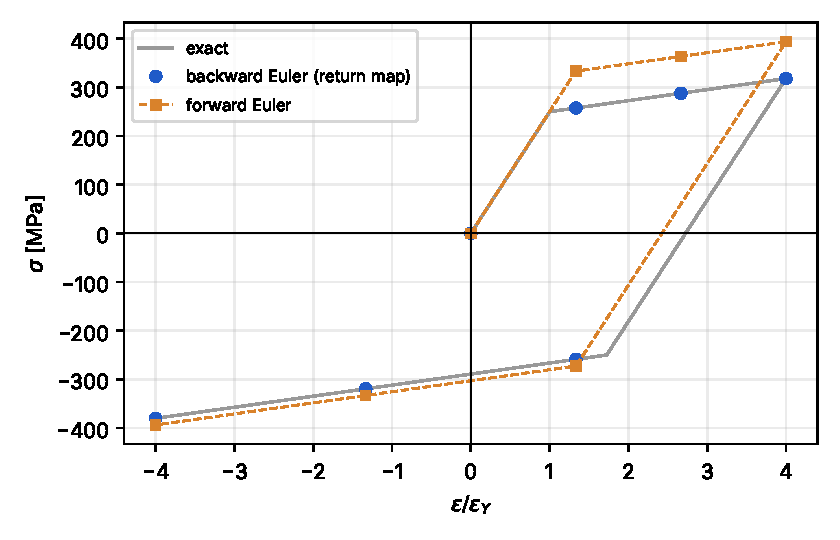
\includegraphics[width=0.62\textwidth]{figures/ch5/euler_filament.pdf}
\caption{Filament with combined hardening ($E=200$\,GPa, $\sY=250$\,MPa,
$K=H=10$\,GPa) under the strain cycle $0\to4\varepsilon_Y\to-4\varepsilon_Y$,
integrated with three steps per branch. Backward Euler (Box~5.1) lies on the
exact curve, the branches being monotone. Forward Euler overshoots the yield
stress in the first step that crosses it, and keeps the error: $393.9$\,MPa
instead of $318.2$\,MPa at the end of the first branch.}
\label{fig:pn-euler}
\end{figure}

%======================================================================
\section{Backward Euler is a closest-point projection}\label{sec:pn-cpp}
\index{closest-point projection}\index{backward Euler!as a projection}%
The plastic corrector of the filament moved the trial state onto the yield
surface. This section shows that, for every generalized standard material, the
corrector is the \emph{projection} of the trial state onto the elastic domain,
in the energy norm of~\eqref{eq:pl-energynorm}. We recall the projection onto
a convex set first~\cite{BauschkeCombettes2017,Moreau1965}.

\subsection{Projection onto a closed convex set}\label{ssec:pn-proj}
\index{projection onto a convex set}\index{non-expansive map}%
Let $X$ be a space with scalar product $\scal{\cdot}{\cdot}$ and norm
$\norm{\cdot}$ (finite dimensional here), and $\mathcal K\subset X$ a nonempty
closed convex set.
\begin{gbox}{Projection onto a convex set}
\begin{itemize}
  \item For every $\vx\in X$ there is a unique $P_{\mathcal K}\vx\in\mathcal K$ closest to $\vx$:
  $\displaystyle P_{\mathcal K}\vx=\argmin_{\vy\in\mathcal K}\tfrac12\norm{\vy-\vx}^2$.
  \item It is characterized by the variational inequality
  \begin{equation}\label{eq:pn-projVI}
    \vp=P_{\mathcal K}\vx\quad\Longleftrightarrow\quad
    \vp\in\mathcal K\ \text{ and }\ \scal{\vx-\vp}{\vy-\vp}\le0\quad\forall\vy\in\mathcal K,
  \end{equation}
  that is, $\vx-\vp$ belongs to the normal cone of $\mathcal K$ at $\vp$, for the
  scalar product $\scal{\cdot}{\cdot}$.
  \item $P_{\mathcal K}$ is \emph{firmly non-expansive}:
  $\norm{P_{\mathcal K}\vx-P_{\mathcal K}\vy}^2\le\scal{P_{\mathcal K}\vx-P_{\mathcal K}\vy}{\vx-\vy}$; in particular
  $\norm{P_{\mathcal K}\vx-P_{\mathcal K}\vy}\le\norm{\vx-\vy}$.
\end{itemize}
\end{gbox}
\paragraph{Why it works.} The squared distance
$\vy\mapsto\tfrac12\norm{\vy-\vx}^2$ is a bowl: strictly convex, and growing
at infinity. On a closed convex set it has exactly one lowest point
(Section~\ref{sec:var-direct}). At that point $\vp$, moving towards any other
point $\vy$ of $\mathcal K$ cannot bring us closer to $\vx$: the angle between
$\vx-\vp$ and $\vy-\vp$ is obtuse, which is~\eqref{eq:pn-projVI}. Draw a
convex body, a point outside and the foot of the perpendicular: every chord
from the foot points away from $\vx$. For the last item, write the angle
condition at $\vp=P_{\mathcal K}\vx$ towards $\vp'=P_{\mathcal K}\vy$, and at
$\vp'$ towards $\vp$, and add the two:
$\scal{(\vx-\vy)-(\vp-\vp')}{\vp'-\vp}\le0$. The Cauchy--Schwarz inequality
gives the Lipschitz bound. Two points are never farther apart than their
shadows on a convex set are close.

\subsection{The return map as a projection}\label{ssec:pn-cpp}
In the generalized variables of Section~\ref{sec:pl-gsm}, the forces are
$\vSig=(\sig,\vq)=-\partial_{\vz}\psi$, and with the quadratic free
energy~\eqref{eq:pl-psi} they are affine in $(\eps,\vz)$:
$\sig=\bbC:(\eps-\epsp)$, $\vq=-\bbD\valpha$. With
$\tensf{G}=\diag(\bbC,\bbD)$, a change $\Delta\vz$ of the internal variables
at fixed strain changes the forces by $-\tensf{G}\Delta\vz$. The \emph{trial
state} freezes the internal variables:
\begin{equation}\label{eq:pn-trial}
  \vSig^\trial_\np=\bigl(\bbC:(\eps_\np-\epsp_n),\ \vq_n\bigr)
  =\vSig_n+\bigl(\bbC:\Delta\eps,\ \vzero\bigr),
  \qquad
  \vSig_\np=\vSig^\trial_\np-\tensf{G}\,\Delta\vz .
\end{equation}
The scalar product of~\eqref{eq:pl-energynorm} is
$\scal{\vSig}{\vSig'}_E=\vSig\cdot\tensf{G}^{-1}\vSig'$, with
$\tensf{G}^{-1}=\diag(\bbS,\bbD^{-1})$: half the squared norm is the
complementary energy, elastic plus hardening.

Now comes the key fact of this chapter. For the filament, the corrector moved
the trial stress straight back to the yield surface. In every dimension, and
for every generalized standard material, it does the same thing: it goes to
the \emph{closest} admissible point.
\begin{gbox}{Backward Euler is a projection}\label{thm:pn-cpp}
The backward Euler step $\Delta\vz\in N_{\Esig}(\vSig_\np)$, with
$\vSig_\np=\vSig^\trial_\np-\tensf{G}\Delta\vz$, has exactly one solution:
the point of the elastic domain closest to the trial state, with the distance
measured in the energy norm,
\begin{equation}\label{eq:pn-cpp}
  \vSig_\np=P^E_{\Esig}\bigl(\vSig^\trial_\np\bigr)
  =\argmin_{\vSig^\ast\in\Esig}\ \tfrac12\norm{\vSig^\ast-\vSig^\trial_\np}_E^2,
  \qquad
  \Delta\vz=\tensf{G}^{-1}\bigl(\vSig^\trial_\np-\vSig_\np\bigr).
\end{equation}
\end{gbox}
\paragraph{Why it works.} Backward Euler asks for a plastic increment
$\Delta\vz$ normal to $\Esig$ at the \emph{end} point $\vSig_\np$: the angle
between $\Delta\vz$ and every chord $\vSig^\ast-\vSig_\np$ of the domain is
obtuse (Section~\ref{ssec:pl-cones}). Replace $\Delta\vz$ by
$\tensf{G}^{-1}(\vSig^\trial_\np-\vSig_\np)$:
\[
  \scal{\vSig^\trial_\np-\vSig_\np}{\vSig^\ast-\vSig_\np}_E\le0\qquad\text{for every }\vSig^\ast\in\Esig .
\]
This is the angle condition~\eqref{eq:pn-projVI} of the closest point, written
in the energy scalar product. The backward Euler equation and the projection
are one and the same equation. The closest point exists and is unique, and so
is the step. Simo and Hughes~\cite{SimoHughesCI} call this algorithm the
\emph{closest-point projection}.

\begin{figure}[h]
\centering
\begin{tikzpicture}[scale=1.15,>=Latex]
  \fill[cu!10,rotate=30] (0,0) ellipse (2.2 and 1.4);
  \draw[thick,cu,rotate=30] (0,0) ellipse (2.2 and 1.4);
  \node[cu] at (-0.5,0.0) {$\Esig$};
  \node[cu] at (-2.2,1.35) {$\partial\Esig$};
  \coordinate (Q) at (0.006,-1.516);
  \coordinate (P) at (1.659,1.376);
  \coordinate (T) at (2.747,2.811);
  \fill (Q) circle (1.6pt) node[below] {$\vSig_n$};
  \draw[->,thick] (Q) .. controls (2.6,-0.9) and (3.2,1.5) .. (T)
    node[pos=0.55,right,font=\small] {$\vSig_n+(\bbC:\Delta\eps,\vzero)$};
  \fill[orange!80!black] (T) circle (1.8pt) node[above right,orange!80!black] {$\vSig^\trial_\np$};
  \draw[->,very thick,orange!80!black] (T) -- ($(P)!0.06!(T)$);
  \fill[cu] (P) circle (1.8pt) node[left=2pt,cu] {$\vSig_\np$};
  \draw[dashed] ($(P)+1.6*(-0.797,0.604)$) -- ($(P)-1.4*(-0.797,0.604)$);
  \draw ($(P)+0.22*(0.604,0.797)$) -- ++($0.22*(-0.797,0.604)$) -- ++($-0.22*(0.604,0.797)$);
  \node[font=\small,orange!80!black,align=left] at (4.3,2.0) {$-\tensf{G}\Delta\vz$\\ (normal to $\partial\Esig$)};
\end{tikzpicture}
\caption{Closest-point projection, after Simo and
Hughes~\cite[Fig.~3.2]{SimoHughesCI}, drawn in coordinates where the energy
norm is Euclidean. The elastic predictor adds $\bbC:\Delta\eps$ to the stress
at fixed internal variables. The plastic corrector returns along the normal to
the yield surface at the \emph{final} point $\vSig_\np$: the trial state is
projected onto the elastic domain.}
\label{fig:pn-cpp}
\end{figure}

The projection is the discrete form of the principle of maximum plastic
dissipation (Section~\ref{thm:pl-maxdiss}): among all admissible forces,
$\vSig_\np$ maximizes $\vSig^\ast\cdot\Delta\vz$. It is also the principle of
minimum complementary energy of one step: the corrector looks for the
admissible force closest to the trial force, in the norm of the energy. Two
consequences are immediate. The elastic step is the case where the trial
state is admissible, since then it is its own projection. And the step
cannot fail: whatever $\Delta\eps$, the discrete problem has exactly one
solution, which is the uniqueness used above for the exactness of the
filament.

When the elastic domain is described by a yield function, the projection
becomes a set of equations that a computer can solve.
\begin{gbox}{Return-mapping equations}\label{cor:pn-rm}
\index{Karush--Kuhn--Tucker conditions!discrete}%
If $\Esig=\{f\le0\}$ with $f$ convex, differentiable and $f(\vzero)<0$, the
projection~\eqref{eq:pn-cpp} is the solution of
\begin{equation}\label{eq:pn-rm}
  \vSig_\np=\vSig^\trial_\np-\dg\,\tensf{G}\,\partial_{\vSig}f(\vSig_\np),\qquad
  \dg\ge0,\quad f(\vSig_\np)\le0,\quad\dg\,f(\vSig_\np)=0 .
\end{equation}
The step is elastic if and only if $f(\vSig^\trial_\np)\le0$.
\end{gbox}
\noindent These are the Karush--Kuhn--Tucker conditions of the minimization
in~\eqref{eq:pn-cpp} (Section~\ref{sec:var-lagrange}), with $\dg$ as the
Lagrange multiplier of the constraint $f\le0$; the condition $f(\vzero)<0$
guarantees that the multiplier exists. An admissible trial state is its own
closest point, which gives $\dg=0$. The first equation contains the backward Euler form of the flow and
hardening rules~\eqref{eq:pl-box-flow}: $\Delta\epsp=\dg\,\partial_{\sig}f$ and
$\Delta\valpha=\dg\,\partial_{\vq}f$, both evaluated at the end of the step. The
normal is the one at the projected point, not at the trial point: this is
what makes the scheme implicit. For a general yield function~\eqref{eq:pn-rm}
is a nonlinear system for $(\vSig_\np,\dg)$, solved by Newton's method on the
active constraint $f(\vSig_\np)=0$~\cite[Sec.~3.2]{SimoHughesCI}; the
\emph{cutting-plane} algorithm of Ortiz and Simo~\cite{OrtizSimo1986} avoids
the second derivatives of $f$ at the price of a linear rate of convergence.
For von Mises the system is solved in closed form.

%======================================================================
\section{\texorpdfstring{$J_2$}{J2} plasticity: radial return and consistent tangent}\label{sec:pn-j2}
\index{radial return}\index{J2 flow theory@$J_2$ flow theory!radial return}%
Take the $J_2$ model~\eqref{eq:pl-j2-f}--\eqref{eq:pl-j2-flow}, with isotropic
elasticity $\bbC=\kappa\,\tI\otimes\tI+2\mu\bbIdev$, linear kinematic hardening
$H$ and an isotropic hardening law $R(\alpha)$, linear ($R=\sY+K\alpha$) or not:
\[
  f(\sig,\tbeta,\alpha)=\norm{\dev\sig-\tbeta}-\sqrt{\tfrac23}\,R(\alpha),\qquad
  \Delta\epsp=\dg\,\tn_\np,\quad \Delta\tbeta=\tfrac23H\dg\,\tn_\np,\quad
  \Delta\alpha=\sqrt{\tfrac23}\,\dg,
\]
with $\tn_\np=\teta_\np/\norm{\teta_\np}$ and $\teta=\dev\sig-\tbeta$. For
this model the projection can be done by hand. The idea goes back to
Wilkins~\cite{Wilkins1964} and to Krieg and Key~\cite{KriegKey1976}.

\begin{gbox}{Radial return}\label{prop:pn-radial}
Let $\tens{s}^\trial=2\mu\dev(\eps_\np-\epsp_n)$,
$\teta^\trial=\tens s^\trial-\tbeta_n$ and
$f^\trial=\norm{\teta^\trial}-\sqrt{2/3}\,R(\alpha_n)$. If $f^\trial>0$, the
corrected state keeps the direction of the trial relative stress and only
shortens it:
\begin{equation}\label{eq:pn-radial}
  \tn_\np=\frac{\teta^\trial}{\norm{\teta^\trial}},\qquad
  \sig_\np=\sig^\trial_\np-2\mu\dg\,\tn_\np,
\end{equation}
where $\dg>0$ is the root of the scalar equation
\begin{equation}\label{eq:pn-radial-g}
  g(\dg):=\norm{\teta^\trial}-\bigl(2\mu+\tfrac23H\bigr)\dg-\sqrt{\tfrac23}\,R\Bigl(\alpha_n+\sqrt{\tfrac23}\dg\Bigr)=0 .
\end{equation}
For linear hardening, $\dg=f^\trial/\bigl(2\mu+\tfrac23(K+H)\bigr)$. The
pressure is not affected: $\tr\sig_\np=\tr\sig^\trial_\np=3\kappa\tr\eps_\np$.
\end{gbox}
\paragraph{Why it works.} Two observations do everything. First, the plastic
strain increment is deviatoric, so the pressure never sees plasticity.
Second, subtract the updates of $\tens s$ and $\tbeta$:
\[
  \teta_\np=\teta^\trial-\bigl(2\mu+\tfrac23H\bigr)\dg\,\tn_\np
  \quad\Longrightarrow\quad
  \Bigl[\norm{\teta_\np}+\bigl(2\mu+\tfrac23H\bigr)\dg\Bigr]\tn_\np=\teta^\trial .
\]
The bracket is a positive number, so the final normal $\tn_\np$ points along
$\teta^\trial$. The normal at the end of the step is known before the step is
computed! The only unknown left is the length $\dg$, and $f_\np=0$
is~\eqref{eq:pn-radial-g}. The function $g$ starts at $g(0)=f^\trial>0$ and
decreases to $-\infty$ ($R$ is non-decreasing): it crosses zero exactly once.

The return is \emph{radial}: in the deviatoric plane, the corrector moves the
trial stress along the radius of the von Mises circle centred at $\tbeta_n$
(Figure~\ref{fig:pn-radial}). It is the projection of
Section~\ref{thm:pn-cpp}: the energy norm on deviators is
$\norm{\tens s}^2/(2\mu)$, proportional to the Euclidean one, and the closest
point of a circle is along the radius. For nonlinear hardening the scalar
equation~\eqref{eq:pn-radial-g} is solved by Newton's method from $\dg=0$;
since $g$ is decreasing and convex for a saturating law (Voce), the iterates
increase monotonically to the root (Exercise~\ref{exo:pn-radial}).

\begin{gbox}{Box 5.2\quad Radial return for \texorpdfstring{$J_2$}{J2} plasticity}
\index{radial return!Box 5.2}%
\begin{enumerate}[label=\textbf{\arabic*.},leftmargin=1.6em]
  \item \textbf{Database.} Read $\epsp_n$, $\tbeta_n$, $\alpha_n$; the strain
  $\eps_\np$ is given.
  \item \textbf{Elastic predictor.}
  \[
    \tens s^\trial=2\mu\dev(\eps_\np-\epsp_n),\qquad
    \teta^\trial=\tens s^\trial-\tbeta_n,\qquad
    f^\trial=\norm{\teta^\trial}-\sqrt{\tfrac23}\,R(\alpha_n).
  \]
  \item \textbf{Check.} If $f^\trial\le0$: $\sig_\np=\kappa(\tr\eps_\np)\tI+\tens s^\trial$,
  internal variables unchanged, tangent $\bbC$; exit.
  \item \textbf{Multiplier.} Solve $g(\dg)=0$, equation~\eqref{eq:pn-radial-g}:
  in closed form for linear hardening, otherwise by Newton,
  \[
    \dg\leftarrow\dg+\frac{g(\dg)}{2\mu+\tfrac23\bigl(H+R'(\alpha_n+\sqrt{2/3}\,\dg)\bigr)} .
  \]
  \item \textbf{Update.} With $\tn=\teta^\trial/\norm{\teta^\trial}$:
  \[
    \sig_\np=\kappa(\tr\eps_\np)\tI+\tens s^\trial-2\mu\dg\,\tn,
  \]
  \[
    \epsp_\np=\epsp_n+\dg\,\tn,\quad
    \tbeta_\np=\tbeta_n+\tfrac23H\dg\,\tn,\quad
    \alpha_\np=\alpha_n+\sqrt{\tfrac23}\,\dg .
  \]
  \item \textbf{Consistent tangent.} Equation~\eqref{eq:pn-calg} below.
\end{enumerate}
\end{gbox}

\begin{figure}[h]
\centering
\begin{tikzpicture}[scale=1.0,>=Latex]
  \begin{scope}
  \fill[cu!10] (0,0) circle (1.8);
  \draw[thick,cu] (0,0) circle (1.8);
  \fill (0,0) circle (1.5pt) node[above left] {$\tbeta_n$};
  \coordinate (T) at (35:3.0);
  \coordinate (P) at (35:1.8);
  \draw[->,thin,gray] (0,0) -- (T);
  \fill[orange!80!black] (T) circle (1.8pt) node[above right,orange!80!black] {$\dev\sig^\trial_\np$};
  \draw[->,very thick,orange!80!black] (T) -- ($(P)!0.05!(T)$);
  \fill[cu] (P) circle (1.8pt) node[left=3pt,cu] {$\dev\sig_\np$};
  \node[font=\small,orange!80!black] at (3.35,1.25) {$-2\mu\dg\,\tn$};
  \draw[<->,gray] (0,0) -- (200:1.8);
  \node[gray,font=\scriptsize] at (-0.75,-0.65) {$\sqrt{\tfrac23}\,R(\alpha_n)$};
  \draw[dashed,cu!70] (0,0) circle (2.05);
  \node[font=\scriptsize,cu!80] at (-1.15,-1.95) {after hardening};
  \node[font=\small] at (0.6,-2.6) {(a) von Mises: radial return};
  \end{scope}
  \begin{scope}[xshift=8.0cm]
  \def\R{1.8}
  \fill[cu!10] (90:\R) -- (30:\R) -- (-30:\R) -- (-90:\R) -- (-150:\R) -- (150:\R) -- cycle;
  \draw[thick,cu] (90:\R) -- (30:\R) -- (-30:\R) -- (-90:\R) -- (-150:\R) -- (150:\R) -- cycle;
  \foreach \a in {90,30,-30,-90,-150,150}{
    \fill[orange!18] (\a:\R) -- ++(\a-30:1.0) arc[start angle=\a-30,end angle=\a+30,radius=1.0] -- cycle;}
  \draw[->,gray] (0,0) -- (90:2.9) node[above,font=\scriptsize] {$\sigma_1$};
  \draw[->,gray] (0,0) -- (210:2.9) node[below left,font=\scriptsize] {$\sigma_2$};
  \draw[->,gray] (0,0) -- (330:2.9) node[below right,font=\scriptsize] {$\sigma_3$};
  % face return
  \coordinate (F) at ($(0:{\R*cos(30)})+(90:0.35)$);
  \coordinate (Ft) at ($(F)+(0:1.1)$);
  \fill[orange!80!black] (Ft) circle (1.6pt);
  \draw[->,very thick,orange!80!black] (Ft) -- ($(F)+(0:0.06)$);
  \fill[cu] (F) circle (1.6pt);
  % corner return
  \coordinate (V) at (90:\R);
  \coordinate (Vt) at ($(V)+(100:0.95)$);
  \fill[orange!80!black] (Vt) circle (1.6pt);
  \draw[->,very thick,orange!80!black] (Vt) -- ($(V)!0.07!(Vt)$);
  \fill[cu] (V) circle (1.6pt);
  \node[font=\scriptsize,align=left] at (3.0,0.9) {face\\ return};
  \node[font=\scriptsize,align=left] at (-1.25,2.55) {corner\\ return};
  \node[font=\small] at (0.3,-2.6) {(b) Tresca: faces and corners};
  \end{scope}
\end{tikzpicture}
\caption{Returns in the deviatoric plane. (a) Von Mises: the corrector is
radial, along $\tn=\teta^\trial/\norm{\teta^\trial}$, onto the circle of
radius $\sqrt{2/3}\,R(\alpha_\np)$. (b) Tresca: a trial state in front of a
face returns along the normal to that face; a trial state in the cone of
normals of a vertex (orange) returns to the vertex
(Section~\ref{sec:pn-multi}).}
\label{fig:pn-radial}
\end{figure}

\subsection{The consistent tangent}\label{ssec:pn-calg}
\index{consistent tangent}\index{tangent modulus!consistent (algorithmic)}%
The return map defines the stress at $t_\np$ as a function of the strain at
$t_\np$, at fixed $\vz_n$. Its derivative
$\bbCalg=\partial\sig_\np/\partial\eps_\np$ is the \emph{consistent} (or
algorithmic) tangent of Simo and Taylor~\cite{SimoTaylor1985}; it is the
matrix that linearizes the discrete global problem
(Section~\ref{sec:pn-newton}). The continuum tangent $\bbCep$
of~\eqref{eq:pl-j2-cep} linearizes the rate equations instead.

\begin{gbox}{Consistent tangent of the radial return}\label{prop:pn-calg}
In a plastic step, with $\theta=1-2\mu\dg/\norm{\teta^\trial}$ and
$\displaystyle \bar\theta=\Bigl(1+\frac{R'(\alpha_\np)+H}{3\mu}\Bigr)^{-1}-(1-\theta)$,
\begin{equation}\label{eq:pn-calg}
  \bbCalg=\kappa\,\tI\otimes\tI+2\mu\theta\,\bbIdev-2\mu\bar\theta\,\tn\otimes\tn .
\end{equation}
It is symmetric, and it tends to the continuum tangent $\bbCep$ as $\dg\to0$.
\end{gbox}
\paragraph{Why it works.} The stress after the return,
$\sig_\np=\kappa(\tr\eps_\np)\tI+\tens s^\trial-2\mu\dg\,\tn$, depends on
$\eps_\np$ through three pieces: the trial deviator, the normal and the
multiplier. Differentiate each piece. The trial deviator gives
$\partial\tens s^\trial/\partial\eps_\np=2\mu\bbIdev$. The normal is a unit
tensor; it can only turn, and the derivative of a unit tensor
(Exercise~\ref{exo:pl-perfect3d}) gives
$\partial\tn/\partial\eps_\np=\dfrac{2\mu}{\norm{\teta^\trial}}\bigl(\bbIdev-\tn\otimes\tn\bigr)$.
The multiplier follows from $g(\dg)=0$, differentiated with
$\partial\norm{\teta^\trial}/\partial\eps_\np=2\mu\tn$:
\[
  2\mu\,\tn-\Bigl(2\mu+\tfrac23H+\tfrac23R'(\alpha_\np)\Bigr)\frac{\partial\dg}{\partial\eps_\np}=\vzero
  \quad\Longrightarrow\quad
  \frac{\partial\dg}{\partial\eps_\np}=\frac{\tn}{1+\frac{R'+H}{3\mu}} .
\]
Collecting,
$\bbCalg=\kappa\tI\otimes\tI+2\mu\bbIdev-2\mu\,\tn\otimes\partial\dg/\partial\eps_\np-2\mu\dg\,\partial\tn/\partial\eps_\np$,
which is~\eqref{eq:pn-calg} after writing $2\mu\dg/\norm{\teta^\trial}=1-\theta$.
Both rank-one terms are dyads of a tensor with itself: the tangent is
symmetric. A vanishing step gives $\theta=1$ and
$\bar\theta=(1+(R'+H)/(3\mu))^{-1}$, which is~\eqref{eq:pl-j2-cep}.
The two tangents differ by the factor $\theta<1$ on the deviatoric directions
orthogonal to $\tn$:
\[
  \bbCalg=\bbCep-2\mu(1-\theta)\bigl(\bbIdev-\tn\otimes\tn\bigr).
\]
The consistent tangent is softer in the directions that rotate the normal. The
reason is geometric: over a finite step, a strain increment orthogonal to
$\tn$ rotates the trial stress, and the radial return then shortens it by
$2\mu\dg$; the continuum tangent, which describes an infinitesimal step, does
not see this. The correction is not small: $1-\theta=2\mu\dg/\norm{\teta^\trial}$
is the fraction of the trial deviator removed by the corrector, close to one
for large steps in perfect plasticity. The eigenvalues of $\bbCalg$ are $3\kappa$
(on $\tI$), $2\mu(\theta-\bar\theta)=2\mu\,\dfrac{R'+H}{3\mu+R'+H}$ (on $\tn$) and $2\mu\theta$
(on the deviators orthogonal to $\tn$); they are positive with hardening.

%======================================================================
\section{The global Newton method}\label{sec:pn-newton}
\index{Newton's method!global equilibrium}%
The global equation~\eqref{eq:pn-residual} is solved by Newton's method. From
an estimate $\mat{u}^{(k)}$, linearize the residual,
$\mat{R}(\mat{u}^{(k)}+\delta\mat{u})\approx\mat{R}(\mat{u}^{(k)})-\mat{K}^{(k)}\delta\mat{u}$,
and solve the linear system
\begin{equation}\label{eq:pn-newton}
  \mat{K}^{(k)}\,\delta\mat{u}=\mat{R}(\mat{u}^{(k)}),\qquad
  \mat{K}^{(k)}=\frac{\partial\mat{F}^{\mathrm{int}}}{\partial\mat{u}}\Bigr|_{\mat{u}^{(k)}}
  =\sum_e\int_{\Omega_e}\mat{B}\T\,\mat{C}^{\mathrm{alg}}\,\mat{B}\dd x,
  \qquad \mat{u}^{(k+1)}=\mat{u}^{(k)}+\delta\mat{u} .
\end{equation}
The tangent stiffness is the derivative of the internal forces, and the chain
rule puts at each Gauss point the derivative of the stress \emph{delivered by
the return map} with respect to the strain: the consistent tangent $\bbCalg$
(in matrix form $\mat{C}^{\mathrm{alg}}$). Newton's method converges
quadratically near the solution only with this matrix~\cite{SimoTaylor1985}.

\begin{gbox}{Box 5.3\quad Incremental elastoplastic computation}
\index{Newton's method!Box 5.3}%
\begin{enumerate}[label=\textbf{\arabic*.},leftmargin=1.6em]
  \item \textbf{Step.} For $n=0,\dots,N-1$: apply the loads and the prescribed
  displacements of $t_\np$; start from $\mat{u}^{(0)}=\mat{u}_n$.
  \item \textbf{Local stage.} At each Gauss point, compute
  $\eps^{(k)}=\mat{B}\mat{u}^{(k)}$ and call the return map
  $(\sig^{(k)},\vz^{(k)},\bbCalg)=\mathcal R(\eps^{(k)};\vz_n)$, always from the
  converged internal variables $\vz_n$ of the previous step.
  \item \textbf{Assembly.}
  $\mat{F}^{\mathrm{int}}=\sum_e\int\mat{B}\T\sig^{(k)}$, $\mat{R}^{(k)}=\mat{F}^{\mathrm{ext}}_\np-\mat{F}^{\mathrm{int}}$,
  $\mat{K}^{(k)}=\sum_e\int\mat{B}\T\mat{C}^{\mathrm{alg}}\mat{B}$.
  \item \textbf{Convergence test.} If $\norm{\mat{R}^{(k)}}\le\mathrm{tol}\,\norm{\mat{F}^{\mathrm{ext}}_\np}$:
  store $\mat{u}_\np=\mat{u}^{(k)}$ and $\vz_\np=\vz^{(k)}$ at every Gauss
  point, and go to the next step.
  \item \textbf{Newton update.} Solve $\mat{K}^{(k)}\delta\mat{u}=\mat{R}^{(k)}$,
  set $\mat{u}^{(k+1)}=\mat{u}^{(k)}+\delta\mat{u}$, and return to stage~2.
\end{enumerate}
\end{gbox}
\noindent Figure~\ref{fig:pn-loop} draws the two nested loops of Box~5.3: the
outer loop on the load steps, and the inner Newton loop, which calls the local
stage at every iteration.

\begin{figure}[h]
\centering
\begin{tikzpicture}[>=Latex,node distance=5mm,
  fbox/.style={rectangle,rounded corners=2pt,fill=gray!12,align=flush center,
    inner sep=4pt,font=\small,text width=#1},fbox/.default=7.6cm,
  test/.style={diamond,aspect=2.6,fill=orange!14,align=flush center,inner sep=1pt,
    font=\small}]
  \node[fbox] (step) {\textbf{1. Step} $n\to n+1$: loads of $t_\np$;\\
    start from $\mat{u}^{(0)}=\mat{u}_n$, $k=0$};
  \node[fbox,kin,below=of step] (loc) {\textbf{2. Local stage}, at each Gauss point:\\
    $(\sig^{(k)},\vz^{(k)},\bbCalg)=\mathcal R\bigl(\mat{B}\mat{u}^{(k)};\,\vz_n\bigr)$};
  \node[fbox,stat,below=of loc] (asm) {\textbf{3. Assembly}:
    $\mat{F}^{\mathrm{int}}$, $\mat{R}^{(k)}=\mat{F}^{\mathrm{ext}}_\np-\mat{F}^{\mathrm{int}}$, $\mat{K}^{(k)}$};
  \node[test,below=of asm] (cv) {\textbf{4.} $\norm{\mat{R}^{(k)}}\le\mathrm{tol}\,\norm{\mat{F}^{\mathrm{ext}}_\np}$\,?};
  \node[fbox=3.7cm,right=8mm of cv] (nw) {\textbf{5. Newton update}\\
    $\mat{K}^{(k)}\delta\mat{u}=\mat{R}^{(k)}$\\ $\mat{u}^{(k+1)}=\mat{u}^{(k)}+\delta\mat{u}$};
  \node[fbox=3.5cm,left=8mm of cv] (acc) {\textbf{Accept}\\
    $\mat{u}_\np=\mat{u}^{(k)}$, $\vz_\np=\vz^{(k)}$\\ at every Gauss point};
  \draw[arr] (step) -- (loc);
  \draw[arr] (loc) -- (asm);
  \draw[arr] (asm) -- (cv);
  \draw[arr] (cv) -- node[above,font=\small] {no} (nw);
  \draw[arr] (cv) -- node[above,font=\small] {yes} (acc);
  \draw[arr] (nw.north) |- node[pos=0.3,right,font=\small,align=left] {$k\gets k+1$\\[-1pt]{\footnotesize\sffamily\color{gray}Newton}} (loc.east);
  \draw[arr] (acc.north) |- node[pos=0.3,left,font=\small,align=right] {$n\gets n+1$\\[-1pt]{\footnotesize\sffamily\color{gray}next step}} (step.west);
\end{tikzpicture}
\caption{The global/local loop of Box~5.3. The local stage (blue) integrates
the flow rule at each Gauss point, always from the converged internal
variables $\vz_n$; the assembly (green) restores equilibrium. The Newton loop
on the right repeats stages 2--5 at fixed $t_\np$; the loop on the left
advances the load step once the residual is small.}
\label{fig:pn-loop}
\end{figure}

\paragraph{Path independence within a step.}
\index{return map!from the converged state}%
The return map in stage~2 starts from $\vz_n$, not from the internal
variables of the previous iterate. The iterates $\mat{u}^{(k)}$ are not states
of the material: they are guesses of the end point of the step, and the
backward Euler step is a function of $(\eps_\np,\vz_n)$ only. Updating the
internal variables from iterate to iterate would make the result depend on the
convergence history and would accumulate spurious plastic strain. Each Gauss
point therefore stores two sets of internal variables: the converged values
of $t_n$ and the current ones.

\paragraph{Consistent against continuum tangent.}
Figure~\ref{fig:pn-newton} compares the two tangents on the thick-walled
cylinder of Exercise~\ref{exo:pl-cyl}, now with Voce hardening and computed
with finite elements (Exercise~\ref{exo:pn-tangent}). With $\bbCalg$ the
residual is squared at each iteration near the solution; with $\bbCep$ it
decreases by a constant factor. Both converge to the same displacement, to
ten digits: the tangent changes the path to the solution, not the solution,
which is fixed by the residual. The first iterations of a step use the elastic
tangent at points that are about to yield, which explains the initial increase
of the residual; a line search on the energy of Section~\ref{sec:pn-var}
prevents it.

\begin{figure}[h]
\centering
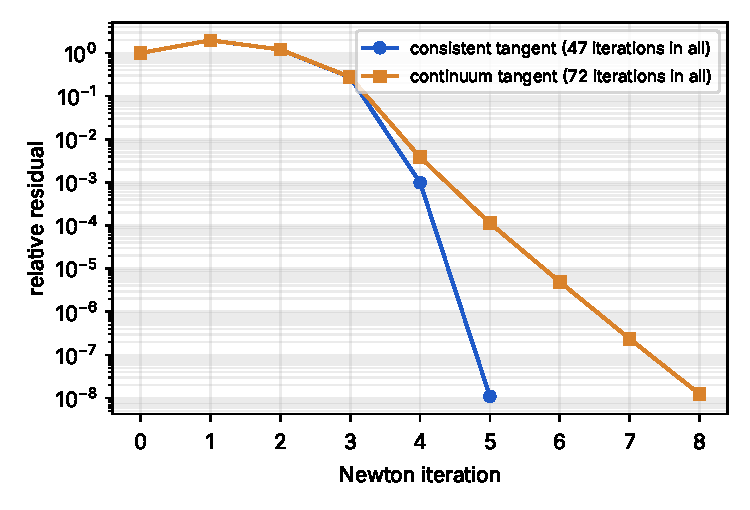
\includegraphics[width=0.6\textwidth]{figures/ch5/newton.pdf}
\caption{Newton iterations in load step 6 of 10 for the thick-walled cylinder
($a=100$, $b=200$\,mm, plane strain, Voce hardening, $p=320$\,MPa, 80
elements). Relative residual against the iteration number with the
consistent tangent (quadratic convergence) and with the continuum tangent
(linear convergence, ratio about $0.05$ per iteration). Over the ten steps
the consistent tangent needs 47 iterations and the continuum one 72.}
\label{fig:pn-newton}
\end{figure}

%======================================================================
\section{Corners: multi-surface plasticity and active sets}\label{sec:pn-multi}
\index{multi-surface plasticity}\index{active set}\index{Tresca criterion!return map}%
When the elastic domain is an intersection of smooth domains,
$\Esig=\bigcap_{\beta=1}^m\{f_\beta\le0\}$ (Tresca, Mohr--Coulomb, crystal
plasticity, caps), the projection property of Section~\ref{thm:pn-cpp} still holds: the solution is the
projection of the trial state. By the last item of the box of
Section~\ref{ssec:pl-cones}, the return-mapping equations~\eqref{eq:pn-rm}
become, with Koiter's rule,
\begin{equation}\label{eq:pn-rm-multi}
  \vSig_\np=\vSig^\trial_\np-\sum_{\beta}\dg^\beta\,\tensf{G}\,\partial_{\vSig}f_\beta(\vSig_\np),\qquad
  \dg^\beta\ge0,\quad f_\beta(\vSig_\np)\le0,\quad\dg^\beta f_\beta(\vSig_\np)=0 .
\end{equation}
The new unknown is the \emph{active set}
$J_\np=\{\beta:\ \dg^\beta>0\}$. It is not, in general, the set of the
surfaces violated by the trial state: a trial state can violate a surface and
return to a point where that surface is inactive. Simo, Kennedy and
Govindjee~\cite{SimoKennedyGovindjee1988} find it by the active-set strategy of
quadratic programming: start from the violated surfaces, solve the projection
with these constraints as equalities, drop the surfaces with a negative
multiplier, add the surfaces violated by the new state, and repeat. Because
the projection is a strictly convex problem, the stress $\vSig_\np$ is unique,
even when the gradients of the active surfaces are linearly dependent and the
multipliers are not.

\paragraph{Tresca in principal stresses.}
For isotropic elasticity and an isotropic criterion, the return does not
rotate the principal axes of the trial stress: the trial deviator, its
projection and the normals are coaxial. The return can therefore be computed
on the ordered principal values $s_1\ge s_2\ge s_3$ of $\sig^\trial_\np$. For
perfect Tresca plasticity the face $f_a=\sigma_1-\sigma_3-\sY$ has the
normal $\tens N_a=\ve_1\otimes\ve_1-\ve_3\otimes\ve_3$ (in the principal
basis), with $\tens N_a:\bbC:\tens N_a=4\mu$. At a vertex two faces are active,
and $\tens N_a:\bbC:\tens N_b=2\mu$ for adjacent faces.

\begin{gbox}{Box 5.4\quad Return map for Tresca (perfect plasticity)}
\index{Tresca criterion!Box 5.4}%
\begin{enumerate}[label=\textbf{\arabic*.},leftmargin=1.6em]
  \item \textbf{Predictor.} Compute $\sig^\trial_\np=\bbC:(\eps_\np-\epsp_n)$, its
  principal values $s_1\ge s_2\ge s_3$ and directions, and $f_a=s_1-s_3-\sY$.
  If $f_a\le0$, the step is elastic.
  \item \textbf{Face return.} $\dg=f_a/(4\mu)$,
  $\sigma_1=s_1-2\mu\dg$, $\sigma_2=s_2$, $\sigma_3=s_3+2\mu\dg$. If
  $\sigma_1\ge\sigma_2\ge\sigma_3$, accept.
  \item \textbf{Corner $\sigma_1=\sigma_2$} (when $s_2>\sigma_1$). With
  $f_b=s_2-s_3-\sY$:
  \[
    \dg^a=\frac{2f_a-f_b}{6\mu},\qquad \dg^b=\frac{2f_b-f_a}{6\mu},
  \]
  \[
    \sigma_1=s_1-2\mu\dg^a,\quad\sigma_2=s_2-2\mu\dg^b,\quad\sigma_3=s_3+2\mu(\dg^a+\dg^b).
  \]
  \item \textbf{Corner $\sigma_2=\sigma_3$} (when $s_2<\sigma_3$). With
  $f_b=s_1-s_2-\sY$ and the same $\dg^a,\dg^b$:
  $\sigma_1=s_1-2\mu(\dg^a+\dg^b)$, $\sigma_2=s_2+2\mu\dg^b$, $\sigma_3=s_3+2\mu\dg^a$.
  \item \textbf{Update.} Rebuild $\sig_\np$ on the principal directions of the
  trial stress, and $\epsp_\np=\epsp_n+\bbS:(\sig^\trial_\np-\sig_\np)$.
\end{enumerate}
\end{gbox}
\noindent The test of stage~2 is the sign of $\dg^b$: the vertex is the
correct return if and only if $2f_b>f_a$, that is, if the trial state lies in
the cone of normals of the vertex (Figure~\ref{fig:pn-radial}b and
Exercise~\ref{exo:pn-tresca}). The return is continuous across the boundary of
that cone, but its derivative is not: the consistent tangent jumps, from a
tangent with one zero eigenvalue (face) to one with two (vertex).

%======================================================================
\section{Plane stress: the projected return}\label{sec:pn-ps}
\index{plane stress!return map}\index{projected return}%
In plates, shells and membranes the stress is plane, $\sigma_{33}=\sigma_{13}=\sigma_{23}=0$,
and the out-of-plane strain $\varepsilon_{33}$ is an unknown. The
three-dimensional radial return cannot be applied directly, because the trial
deviator would need $\varepsilon_{33}$. One option is to iterate on
$\varepsilon_{33}$ until $\sigma_{33}=0$ around the three-dimensional return.
Simo and Taylor~\cite{SimoTaylor1986} work instead in the plane-stress subspace,
with the vectors $\vect{\sigma}=(\sigma_{11},\sigma_{22},\sigma_{12})$ and
$\vect{\varepsilon}=(\varepsilon_{11},\varepsilon_{22},2\varepsilon_{12})$, the
plane-stress moduli and the von Mises matrix
\[
  \mat{C}=\frac{E}{1-\nu^2}\begin{bmatrix}1&\nu&0\\ \nu&1&0\\ 0&0&\tfrac{1-\nu}{2}\end{bmatrix},
  \qquad
  \mat{P}=\frac13\begin{bmatrix}2&-1&0\\ -1&2&0\\ 0&0&6\end{bmatrix},
  \qquad
  \vect{\sigma}\T\mat{P}\vect{\sigma}=\norm{\dev\sig}^2=2J_2 .
\]
For isotropic hardening the yield function is
$f=\tfrac12\vect{\sigma}\T\mat{P}\vect{\sigma}-\tfrac13R(\alpha)^2$, and the
backward Euler step reads
\begin{equation}\label{eq:pn-ps}
  \vect{\sigma}_\np=\vect{\sigma}^\trial_\np-\dg\,\mat{C}\mat{P}\vect{\sigma}_\np
  \quad\Longrightarrow\quad
  \vect{\sigma}_\np=\bigl(\mat{I}+\dg\,\mat{C}\mat{P}\bigr)^{-1}\vect{\sigma}^\trial_\np,
  \quad
  \alpha_\np=\alpha_n+\sqrt{\tfrac23}\,\dg\,\varphi(\dg),
\end{equation}
with $\varphi=\sqrt{\vect{\sigma}_\np\T\mat{P}\vect{\sigma}_\np}=\norm{\dev\sig_\np}$.
The return is \emph{not} radial: $\mat{C}\mat{P}$ is not a multiple of the
identity. But $\mat{C}$ and $\mat{P}$ have the same eigenvectors,
$(1,1,0)/\sqrt2$, $(-1,1,0)/\sqrt2$ and $(0,0,1)$, with eigenvalues
$E/(1-\nu)$, $2\mu$, $\mu$ for $\mat{C}$ and $\tfrac13$, $1$, $2$ for
$\mat{P}$. In this basis the inverse is diagonal, and the whole return
reduces to one scalar equation (Exercise~\ref{exo:pn-ps}).
Figure~\ref{fig:pn-ps} shows the return in the plane of the principal
stresses. The yield locus is the ellipse
$\sigma_{11}^2-\sigma_{11}\sigma_{22}+\sigma_{22}^2=\sY^2$. A uniaxial trial
stress does not return to the uniaxial point: the corrector follows
$\mat{C}\mat{P}\vect{\sigma}_\np$, which is the normal in the energy norm but
neither the radius nor the Euclidean normal $\mat{P}\vect{\sigma}_\np$.

\begin{gbox}{Box 5.5\quad Projected return for plane stress}
\index{plane stress!Box 5.5}%
\begin{enumerate}[label=\textbf{\arabic*.},leftmargin=1.6em]
  \item \textbf{Predictor.} $\vect{\sigma}^\trial=\mat{C}(\vect{\varepsilon}_\np-\vect{\varepsilon}^p_n)$;
  if $\tfrac12\vect{\sigma}^{\trial\top}\mat{P}\vect{\sigma}^\trial\le\tfrac13R(\alpha_n)^2$, the step is elastic.
  \item \textbf{Modes.} For $\dg\ge0$,
  \[
    \varphi^2(\dg)=\frac{(\sigma^\trial_{11}+\sigma^\trial_{22})^2}{6\bigl(1+\frac{E\dg}{3(1-\nu)}\bigr)^2}
    +\frac{\tfrac12(\sigma^\trial_{22}-\sigma^\trial_{11})^2+2(\sigma^\trial_{12})^2}{(1+2\mu\dg)^2}.
  \]
  \item \textbf{Consistency.} Solve the scalar equation
  $\tfrac12\varphi^2(\dg)-\tfrac13R^2\bigl(\alpha_n+\sqrt{2/3}\,\dg\,\varphi(\dg)\bigr)=0$
  for $\dg>0$ (Newton, or bisection).
  \item \textbf{Update.} $\vect{\sigma}_\np=(\mat{C}^{-1}+\dg\mat{P})^{-1}\mat{C}^{-1}\vect{\sigma}^\trial$,
  $\vect{\varepsilon}^p_\np=\vect{\varepsilon}^p_n+\dg\,\mat{P}\vect{\sigma}_\np$,
  $\alpha_\np=\alpha_n+\sqrt{2/3}\,\dg\,\varphi(\dg)$; the thickness strain
  follows from $\sigma_{33}=0$.
\end{enumerate}
\end{gbox}
\noindent The plane-stress condition is satisfied exactly, without nested
iterations, which makes Box~5.5 the standard algorithm of shell elements. Its
consistent tangent is given in~\cite[Box~3.4]{SimoHughesCI}.

\begin{figure}[h]
\centering
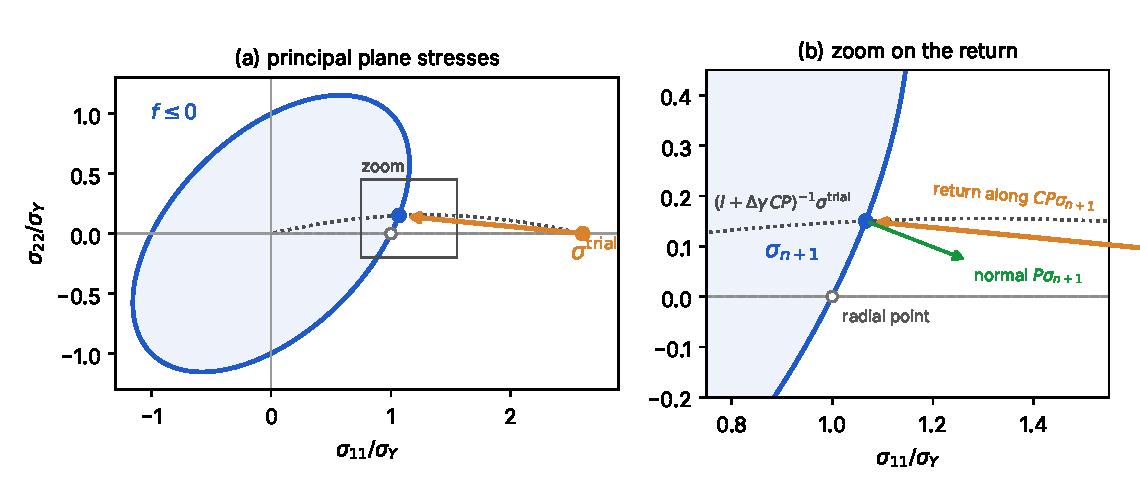
\includegraphics[width=\textwidth]{figures/ch5/plane_stress_return.pdf}
\caption{Projected return in plane stress (Box~5.5), perfect plasticity,
$\nu=0.3$, principal stresses ($\sigma_{12}=0$). (a) The trial stress
$\sigma^\trial=2.6\,\sY$ is uniaxial. The solution is sought on the curve
$\dg\mapsto(\mat{I}+\dg\,\mat{C}\mat{P})^{-1}\vect{\sigma}^\trial$ (dotted), which
crosses the ellipse at $\vect{\sigma}_\np=(1.067,\,0.150)\,\sY$; the radial
point $(1,0)\,\sY$ is not the solution. (b) Zoom: the straight return
$\vect{\sigma}^\trial-\vect{\sigma}_\np=\dg\,\mat{C}\mat{P}\vect{\sigma}_\np$
is not along the Euclidean normal $\mat{P}\vect{\sigma}_\np$ (green).}
\label{fig:pn-ps}
\end{figure}

%======================================================================
\section{Viscoplasticity}\label{sec:pn-vp}
\index{viscoplasticity!return map}%
In viscoplasticity the flow rule is a differential equation with a finite
right-hand side (Section~\ref{ssec:pl-gsm-def}), and backward Euler keeps the
time step.

\paragraph{Perzyna.}
\index{viscoplasticity!Perzyna}%
With the dual potential~\eqref{eq:pl-perzyna},
$\dot\vz=\eta^{-1}\mac{f(\vSig)}\,\partial_{\vSig}f$, the discrete multiplier
is no longer fixed by $f_\np=0$ but by
\begin{equation}\label{eq:pn-perzyna}
  \dg=\frac{\Delta t}{\eta}\,f(\vSig_\np)\qquad\text{(plastic step)}:
\end{equation}
the overstress at the end of the step is proportional to the multiplier. For
$J_2$ plasticity with linear hardening the radial return applies unchanged,
with
\begin{equation}\label{eq:pn-perzyna-j2}
  \dg=\frac{f^\trial}{2\mu+\tfrac23(K+H)+\eta/\Delta t} .
\end{equation}
The rate-independent return is recovered for $\eta\to0$, and also for
$\Delta t\to\infty$ at fixed $\eta$: over a long step the overstress has time to
relax. For $\eta/\Delta t$ large compared with $2\mu$, the step is nearly
elastic. The consistent tangent~\eqref{eq:pn-calg} holds with $R'+H$ replaced
by $R'+H+\tfrac32\eta/\Delta t$.

\paragraph{Duvaut--Lions.}
\index{viscoplasticity!Duvaut--Lions}%
The Duvaut--Lions model of Section~\ref{ssec:pl-gsm-def} relaxes the forces
towards their projection onto $\Esig$:
$\dot\vz=\tau^{-1}\tensf{G}^{-1}\bigl(\vSig-P^E_{\Esig}\vSig\bigr)$, with the
relaxation time $\tau$. Its backward Euler step is a simple modification of
the rate-independent one~\cite[Sec.~2.7]{SimoHughesCI}.
\begin{gbox}{Duvaut--Lions update}\label{prop:pn-dl}
Let $r=\Delta t/\tau$ and let $\bar\vSig_\np=P^E_{\Esig}(\vSig^\trial_\np)$ be
the rate-independent solution. The viscoplastic state lies on the segment
from the trial state to its projection:
\begin{equation}\label{eq:pn-dl}
  \vSig_\np=\frac{\vSig^\trial_\np+r\,\bar\vSig_\np}{1+r},
\end{equation}
and this is the only solution of the backward Euler step.
\end{gbox}
\paragraph{Why it works.} Look at Figure~\ref{fig:pn-dl}. With $P=P^E_{\Esig}$,
backward Euler asks $\tensf{G}\Delta\vz=r(\vSig_\np-P\vSig_\np)$, that is,
$(1+r)\vSig_\np-rP\vSig_\np=\vSig^\trial_\np$. Try a point on the segment
from $\bar\vSig_\np$ to the trial state. All the points of that segment have
the same closest point $\bar\vSig_\np$: sliding along the normal does not move
the foot of the perpendicular (this is~\eqref{eq:pn-projVI}). So
$P\vSig_\np=\bar\vSig_\np$, the equation becomes linear,
$(1+r)\vSig_\np-r\bar\vSig_\np=\vSig^\trial_\np$, and its solution
is~\eqref{eq:pn-dl}. There is no other solution: subtract the equations of two
solutions and use that $I-P$ is monotone (firm non-expansiveness); this gives
$(1+r)\norm{\vSig-\vSig'}_E^2-r\norm{\vSig-\vSig'}_E^2\le0$.
The viscoplastic state lies on the segment between the trial state ($r\to0$,
a very viscous or a very short step) and the projection ($r\to\infty$)
(Figure~\ref{fig:pn-dl}). Its distance to $\Esig$, the overstress, is the fraction
$\displaystyle \frac{1}{1+r}$ of the distance of the trial state. A
viscoplastic code is obtained from a plastic one with two extra lines.

\begin{figure}[h]
\centering
\begin{tikzpicture}[scale=1.1,>=Latex]
  \fill[cu!10] (0,0) ellipse (2.0 and 1.3);
  \draw[thick,cu] (0,0) ellipse (2.0 and 1.3);
  \node[cu] at (-0.6,-0.1) {$\Esig$};
  % P on the boundary (parameter 15 deg), unit normal n, perpendicular m
  \coordinate (P) at (1.932,0.336);
  \def\nx{0.925}\def\ny{0.381}
  \coordinate (T) at ($(P)+4.2*(\nx,\ny)$);
  \coordinate (S) at ($(P)!0.4!(T)$);
  \draw[dashed,gray] ($(P)+0.9*(-\ny,\nx)$) -- ($(P)-0.6*(-\ny,\nx)$);
  \draw[very thick,orange!80!black] (P) -- (T);
  \fill[orange!80!black] (T) circle (1.8pt) node[right=3pt,orange!80!black,align=left]
    {$\vSig^\trial_\np$\\ ($r\to0$)};
  \fill[cu] (P) circle (1.8pt) node[below right=6pt and 4pt,cu,align=left]
    {$\bar\vSig_\np=P^E_{\Esig}\vSig^\trial_\np$\\ ($r\to\infty$, plasticity)};
  \fill (S) circle (2.1pt) node[below right=2pt and 0pt] {$\vSig_\np$};
  \draw[decorate,decoration={brace,amplitude=5pt},thick,gray]
    ($(P)+0.15*(-\ny,\nx)$) -- ($(S)+0.15*(-\ny,\nx)$);
  \draw[decorate,decoration={brace,amplitude=5pt},thick,gray]
    ($(S)+0.15*(-\ny,\nx)$) -- ($(T)+0.15*(-\ny,\nx)$);
  \node[font=\small] at ($(P)!0.5!(S)+0.88*(-\ny,\nx)$) {$\dfrac{1}{1+r}$};
  \node[font=\small] at ($(S)!0.5!(T)+0.88*(-\ny,\nx)$) {$\dfrac{r}{1+r}$};
\end{tikzpicture}
\caption{Duvaut--Lions update~\eqref{eq:pn-dl}, drawn in coordinates where the
energy norm is Euclidean. The viscoplastic state is a point of the segment
joining the trial state to its projection $\bar\vSig_\np$ on the elastic
domain, with $r=\Delta t/\tau$; the brace labels are the fractions of the
length of the segment. Every point of the segment projects onto
$\bar\vSig_\np$, which is why the update needs only the rate-independent
return.}
\label{fig:pn-dl}
\end{figure}

%======================================================================
\section{Accuracy and stability}\label{sec:pn-stab}
\index{return map!accuracy}\index{return map!stability}\index{B-stability}%
\paragraph{Accuracy.}
\index{iso-error map}%
Backward Euler is first-order accurate: the local error over a step is
$O(\Delta t^2)$, the global error $O(\Delta t)$~\cite{OrtizPopov1985,SimoHughesCI}.
For the radial return the error comes from the rotation of the normal: the
exact solution integrates $\dot\epsp=\gamma\tn(t)$ with a turning $\tn$, the
algorithm uses the final normal for the whole step. The error vanishes when
the normal does not turn. Hence the radial return is exact on
\emph{proportional} paths with linear hardening (simple shear, uniaxial
tension, the filament on monotone steps), whatever the step size, and first
order on non-proportional paths (Exercise~\ref{exo:pn-shear}). The error over
one step is mapped by the \emph{iso-error maps} of Krieg and
Krieg~\cite{KriegKrieg1977} and Simo and Taylor~\cite{SimoTaylor1985}
(Figure~\ref{fig:pn-isoerror}): a strain increment along the normal produces
no error, an increment along the tangent the largest one. A useful rule
follows: steps of a few yield strains are acceptable on proportional
parts of a loading, and must be refined where the loading path turns. A
code that reproduces all the proportional calibration tests (tension, simple
shear, balanced biaxial tension) at one step per increment is correctly
programmed, but its step size is not validated.

\begin{figure}[h]
\centering
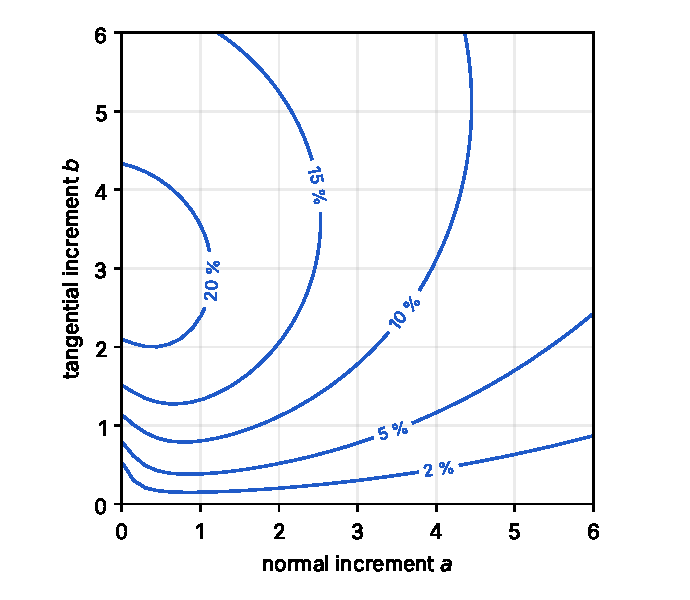
\includegraphics[width=0.5\textwidth]{figures/ch5/isoerror.pdf}
\caption{Iso-error map of the radial return, perfect $J_2$ plasticity, after
Simo and Taylor~\cite{SimoTaylor1985}. The initial state is on the yield
surface in uniaxial tension; one step of strain increment
$\Delta\eps=(a\,\tn+b\,\tens t)\,R/(2\mu)$, with $\tens t$ a unit deviator
orthogonal to $\tn$ and $R=\sqrt{2/3}\,\sY$, is compared with a solution with
1000 sub-steps. Contours: relative error on the deviatoric stress. The error
is zero for a normal increment ($b=0$) and largest for a tangential increment
of a few yield strains ($22\,\%$ at $a=0$, $b=3$).}
\label{fig:pn-isoerror}
\end{figure}

Second-order accuracy is obtained by the generalized midpoint rule, which
evaluates the normal at an intermediate point of the step; it is stable for
the midpoint parameter $\alpha\ge\tfrac12$ and second order for
$\alpha=\tfrac12$, but it gives up the projection structure and its
properties~\cite{OrtizPopov1985,SimoGovindjee1991}. In practice, step-size
control is preferred.

\paragraph{Stability.}
Plasticity is dissipative: two solutions driven by the same strain history do
not move apart in the energy norm (the argument for the uniqueness of the
stresses, Section~\ref{thm:pl-unique}, at a single point). A good algorithm
keeps this property for every step size.

\begin{gbox}{The return map never increases distances}\label{thm:pn-contract}
Drive two states $\vSig_n$ and $\vSig'_n$ with the same strain increment
$\Delta\eps$. After the return map they are not farther apart, in the energy
norm:
\[
  \norm{\vSig_\np-\vSig'_\np}_E\le\norm{\vSig_n-\vSig'_n}_E ,
\]
whatever the size of the step.
\end{gbox}
\paragraph{Why it works.} Two lines. The elastic predictor adds the same
$(\bbC:\Delta\eps,\vzero)$ to both states~\eqref{eq:pn-trial}, so the trial
states are exactly as far apart as the old states. The corrector projects
both onto the same convex set (Section~\ref{thm:pn-cpp}), and projections
never increase distances (Section~\ref{ssec:pn-proj}). Simo and
Govindjee~\cite{SimoGovindjee1991} call this property \emph{contractivity}.

The bound holds for every $\Delta\eps$: the return map is unconditionally
stable in the nonlinear sense (B-stability). Errors made in a step, for
instance by a loose tolerance of the global Newton iterations, are not
amplified by the following steps. Forward Euler has no such property. Take the
perfectly plastic filament with one state on the yield surface, $\sigma=\sY$,
and one inside, $\sigma'=\sY-\delta$, and a strain increment
$\Delta\varepsilon>2\delta/E$: forward Euler leaves $\sigma$ unchanged and
moves $\sigma'$ elastically to $\sY-\delta+E\Delta\varepsilon$, so that the
distance grows from $\delta$ to $E\Delta\varepsilon-\delta$; the return map
gives $\sigma_\np=\sigma'_\np=\sY$ (Exercise~\ref{exo:pn-contract}).

%======================================================================
\section{The incremental problem as a minimization}\label{sec:pn-var}
\index{variational constitutive update}\index{incremental potential}%
The projection of Section~\ref{thm:pn-cpp} describes the step by a
minimization over the \emph{forces}. The same step is also a minimization over
the \emph{internal variables}, and that one gives an energy for the whole
incremental problem. Here is the idea in words: one step of plasticity
chooses the internal variables that make the stored energy plus the
dissipated energy as small as possible. This is the variational constitutive
update of Ortiz and Stainier~\cite{OrtizStainier1999}; see
also~\cite{Miehe2002} and~\cite[Sec.~2.8]{KondoMaitournam2023b}.

\begin{gbox}{One step minimizes stored plus dissipated energy}\label{thm:pn-W}
For the quadratic free energy~\eqref{eq:pl-psi} and $\Esig$ closed convex with
$\vzero\in\Esig$, let
\begin{equation}\label{eq:pn-Wn}
  W_n(\eps)=\min_{\vz}\Bigl\{\psi(\eps,\vz)-\psi(\eps_n,\vz_n)+\pi_{\Esig}(\vz-\vz_n)\Bigr\},
\end{equation}
the change of free energy plus the dissipation of the step, minimized over the
internal variables. Then:
\begin{enumerate}[label=(\alph*)]
  \item the minimizer is $\vz_\np=\vz_n+\Delta\vz$, the backward Euler step;
  \item $W_n(\eps)=\psi(\eps,\vz_n)-\psi(\eps_n,\vz_n)-\tfrac12\,\mathrm{dist}_E\bigl(\vSig^\trial(\eps),\Esig\bigr)^2$;
  \item $W_n$ is convex and differentiable, and
  $\partial W_n/\partial\eps=\sig_\np$: the return map derives from a potential;
  \item where $W_n$ is twice differentiable,
  $\bbCalg=\partial^2W_n/\partial\eps^2$ is symmetric and positive
  semi-definite.
\end{enumerate}
\end{gbox}
\paragraph{Why it works.} (a) Write the increment as $\vect\zeta=\vz-\vz_n$.
Because $\psi$ is quadratic in $\vz$, the function to minimize is a bowl plus
the dissipation,
$\Phi(\vect\zeta)=\tfrac12\vect\zeta\cdot\tensf{G}\vect\zeta-\vSig^\trial\cdot\vect\zeta+\pi_{\Esig}(\vect\zeta)$,
up to a constant. At the bottom the slopes balance:
$\vSig^\trial-\tensf{G}\vect\zeta\in\partial\pi_{\Esig}(\vect\zeta)$. The force
at the end of the step is a slope of the dissipation function at the
increment. By the principle of maximum dissipation (Section~\ref{thm:pl-maxdiss},
forms (b) and (c)) this says that $\vect\zeta$ is normal to $\Esig$ at
$\vSig^\trial-\tensf{G}\vect\zeta$: it is the backward Euler step.
(b) At the bottom, the dissipation equals $\vSig_\np\cdot\Delta\vz$ (form (d)
of the same principle), and $\vSig_\np=\vSig^\trial-\tensf{G}\Delta\vz$, so
$\Phi(\Delta\vz)=-\tfrac12\Delta\vz\cdot\tensf{G}\Delta\vz=-\tfrac12\norm{\vSig^\trial-\vSig_\np}_E^2$.
(c) Minimizing a jointly convex function of $(\eps,\vz)$ over $\vz$ leaves a
convex function of $\eps$. For the gradient, the gradient of half a squared
distance to a convex set is the gap $\vSig-P^E_{\Esig}\vSig$, and the chain
rule gives
$\partial W_n/\partial\eps=\sig^\trial-\bbC:\bbS:(\sig^\trial-\sig_\np)=\sig_\np$.
(d) A Hessian is always symmetric, and it is positive semi-definite for a
convex function.

The last item is the general reason for the symmetry of the consistent
tangent~\eqref{eq:pn-calg}: the return map of an associative model is the
gradient of a convex potential. For a non-associative model there is no such
potential, and the tangent is not symmetric (Exercise~\ref{exo:pn-hill}).

\begin{example}[$J_2$ plasticity and the filament]\label{ex:pn-WJ2}
For the radial return with linear hardening, $\Delta\vz$ is $\dg$ times the
normal and $\mathrm{dist}_E^2=\Delta\vz\cdot\tensf{G}\Delta\vz=h\,\dg^2$ with
$h=2\mu+\tfrac23(K+H)$. Hence
\begin{equation}\label{eq:pn-WJ2}
  W_n(\eps)=\psi(\eps,\vz_n)-\psi(\eps_n,\vz_n)-\frac{\mac{f^\trial(\eps)}^2}{2h} ,
\end{equation}
the elastic trial energy minus a correction that switches on at yield. Its
Hessian in the plastic region is~\eqref{eq:pn-calg}. For the virgin filament,
$W_0(\varepsilon)=\tfrac12E\varepsilon^2-\mac{E|\varepsilon|-\sY}^2/(2(E+K+H))$
(Figure~\ref{fig:pn-W1d}): its derivative is the bilinear response of one
step. Without hardening, $W_0$ grows only linearly at infinity.
\end{example}

\begin{figure}[h]
\centering
\begin{tikzpicture}[scale=0.85,>=Latex]
  \begin{scope}
  \draw[->] (-3.2,0) -- (3.4,0) node[right] {$\varepsilon/\varepsilon_Y$};
  \draw[->] (0,-0.3) -- (0,4.8) node[above] {$W_0$};
  \draw[dashed,gray,thick,domain=-3:3,samples=60] plot (\x,{0.5*\x*\x});
  \draw[very thick,cu,domain=-3:3,samples=121] plot (\x,{0.5*\x*\x-(max(abs(\x)-1,0))^2/(2*1.25)});
  \node[gray,font=\small] at (2.0,4.3) {$\tfrac12E\varepsilon^2$};
  \end{scope}
  \begin{scope}[xshift=8cm,yshift=2.2cm]
  \draw[->] (-3.2,0) -- (3.4,0) node[right] {$\varepsilon/\varepsilon_Y$};
  \draw[->] (0,-2.2) -- (0,2.4) node[above] {$\sigma/\sY=W_0'$};
  \draw[dashed,gray,thick,domain=-2.1:2.1] plot (\x,{\x});
  \draw[very thick,orange!80!black,domain=-3:3,samples=121] plot (\x,{\x-sign(\x)*max(abs(\x)-1,0)/1.25});
  \end{scope}
\end{tikzpicture}
\caption{Incremental potential of the virgin filament (left) and its
derivative, the stress after one step (right), for $(K+H)/E=0.25$. The
curvature drops from $E$ to $E(K+H)/(E+K+H)$ at yield.}
\label{fig:pn-W1d}
\end{figure}

\paragraph{The global problem.}
\index{minimum principle!incremental}%
Summing over the body, the incremental problem~\eqref{eq:pn-global}--\eqref{eq:pn-local}
is the minimization of
\begin{equation}\label{eq:pn-Pi}
  \Pi_n(\vu)=\int_\Omega W_n\bigl(\vx,\eps[\vu]\bigr)\dd x-\ell_\np(\vu),
  \qquad \vu\in\Kad(\vuD(t_\np),S_u),
\end{equation}
where $W_n(\vx,\cdot)$ is built with the internal variables $\vz_n(\vx)$: its
stationarity condition is the weak equilibrium~\eqref{eq:pn-global} with
$\sig_\np=\partial W_n/\partial\eps$. With hardening, $W_n$ is strongly convex
(its Hessian is bounded below by
$\min\{3\kappa,\ 2\mu(K+H)/(3\mu+K+H)\}$), and $\Pi_n$ has a unique minimizer, by
the direct method of Section~\ref{sec:var-direct} and Korn's inequality. The
incremental elastoplastic problem is thus a nonlinear elasticity problem, with
a potential that changes from step to step. Newton's method of Box~5.3 is
Newton's method for this minimization; its matrix, the Hessian of $\Pi_n$, is
symmetric, and a line search on $\Pi_n$ makes it globally convergent. Without
hardening, $W_n$ has linear growth, the minimization is not coercive in $H^1$,
and the solution may develop the discontinuities of
Section~\ref{ssec:pl-unique}. Minimizing $\Pi_n$ over a representative volume
of a heterogeneous material defines an effective incremental potential, which
is the incremental variational homogenization of Miehe~\cite{Miehe2002}.

%======================================================================
\framepart{Summary}
\begin{gbox*}
\begin{itemize}
  \item \textbf{The incremental problem} alternates a global, linear
  equilibrium (assembled and solved by Newton's method) and a local, nonlinear
  integration of the flow rule at each Gauss point, always from the converged
  internal variables $\vz_n$ of the previous step.
  \item \textbf{The return map} is backward Euler: an elastic predictor
  $\vSig^\trial=\vSig_n+(\bbC:\Delta\eps,\vzero)$, a check
  $f(\vSig^\trial)\le0$, and a plastic corrector. For the filament
  $\dg=f^\trial/(E+K+H)$, exact on monotone steps.
  \item \textbf{Closest-point projection:} the corrector projects the trial
  state onto $\Esig$ in the complementary energy norm. The discrete solution
  exists, is unique, and is the discrete form of maximum dissipation.
  \item \textbf{Radial return} for $J_2$ plasticity:
  $\tn=\teta^\trial/\norm{\teta^\trial}$, $\sig_\np=\sig^\trial-2\mu\dg\,\tn$,
  $\dg=f^\trial/(2\mu+\tfrac23(K+H))$ for linear hardening, a scalar Newton
  iteration otherwise.
  \item \textbf{The consistent tangent}
  $\bbCalg=\kappa\tI\otimes\tI+2\mu\theta\bbIdev-2\mu\bar\theta\,\tn\otimes\tn$
  is the derivative of the return map; it differs from $\bbCep$ and is needed
  for the quadratic convergence of the global Newton method.
  \item \textbf{Corners, plane stress, viscosity:} active-set strategy (closed
  form for Tresca), projected return with one scalar equation, Perzyna
  ($\dg=\Delta t f_\np/\eta$) and Duvaut--Lions (segment between trial state
  and projection).
  \item \textbf{Accuracy and stability:} first order, exact on proportional
  paths, unconditionally contractive in the energy norm (projections are
  non-expansive). Forward Euler drifts and is not contractive.
  \item \textbf{Variational form:} the step minimizes stored plus dissipated
  energy; the incremental potential $W_n$ is convex, $\sig_\np=\partial W_n/\partial\eps$,
  $\bbCalg=\partial^2W_n/\partial\eps^2$, and the incremental structural
  problem is the minimization of $\Pi_n$.
\end{itemize}
\end{gbox*}

\framepart{Exercises}\label{sec:pn-exo}
The exercises follow the chapter. Short questions without computer come
first, in the format of a written exam. Then come the filament by hand,
$J_2$ plasticity, corners and plane stress, stability and the variational
form, and a finite element code. The computational exercises use two
auxiliary Python modules, presented on page~\pageref{sec:pn-aux}:
\texttt{ci\_core}, which contains the return maps of Boxes~5.1--5.5 and their
tangents, and \texttt{ci\_fem}, a small finite element driver for the global
Newton method of Box~5.3. Each exercise says which of them it uses. The
results are stated in words first, and the scripts are printed after them.
Solutions are given in small type after each exercise.

\framesub{Short questions}
The questions below need no documents and no computer: a few lines of
algebra and a pocket calculation each.

\exercise{One step of the filament}\label{exo:pn-q-filament}
\index{return map!filament (exercise)}%
A virgin filament has $E=200$\,GPa, $\sY=200$\,MPa and linear isotropic
hardening $K=20$\,GPa ($H=0$). (a) Compute, in one step of Box~5.1, the
stress, the plastic strain and $\alpha$ at $\varepsilon=0.003$. (b) The
strain is then decreased by $0.001$ in one step. Is the step elastic?
\begin{solution}
(a) $\sigma^\trial=600$\,MPa, $f^\trial=400$\,MPa,
$\dg=400/220\,000=1.818\times10^{-3}$, so
$\varepsilon^p=\alpha=1.818\times10^{-3}$ and
$\sigma=600-200\,000\times1.818\times10^{-3}=236.4$\,MPa, which is
$\sY+K\alpha$. (b) $\sigma^\trial=236.4-200=36.4$\,MPa and
$f^\trial=36.4-236.4<0$: the step is elastic, and $\sigma=36.4$\,MPa.
\end{solution}

\exercise{Radial return by hand}\label{exo:pn-q-radial}
\index{radial return!exercise}%
Perfect $J_2$ plasticity, $\mu=80$\,GPa, $\sY=240$\,MPa. A trial deviator
has the norm $\norm{\tens s^\trial}=1.5\sqrt{2/3}\,\sY$. (a) Compute $\dg$,
the norm of the plastic strain increment, and the fraction of the trial
deviator removed by the corrector. (b) Compute the eigenvalue of $\bbCalg$ on
the deviators orthogonal to $\tn$, and compare with $\bbCep$.
\begin{solution}
(a) $\sqrt{2/3}\,\sY=195.96$\,MPa, $\norm{\tens s^\trial}=293.94$\,MPa,
$f^\trial=97.98$\,MPa and $\dg=f^\trial/(2\mu)=6.12\times10^{-4}$. This is
also $\norm{\Delta\epsp}$, since $\tn$ is a unit tensor. The corrector removes
the fraction $2\mu\dg/\norm{\tens s^\trial}=1/3$ of the trial deviator.
(b) $\theta=2/3$, and the eigenvalue is $2\mu\theta=106.7$\,GPa, instead of
$2\mu=160$\,GPa for $\bbCep$: the consistent tangent is softer in the
directions that rotate the normal.
\end{solution}

\exercise{Reading a convergence history}\label{exo:pn-q-newton}
\index{consistent tangent!exercise}%
Two computations of the same load step give the relative residuals
(A) $10^{-1}$, $10^{-2}$, $10^{-4}$, $10^{-8}$ and (B) $10^{-1}$,
$5\times10^{-3}$, $2.5\times10^{-4}$, $1.25\times10^{-5}$. Which one uses the
consistent tangent? How many more iterations does (B) need to reach
$10^{-10}$? Do the two converged solutions differ?
\begin{solution}
(A): the exponent doubles at each iteration. This is quadratic convergence,
obtained with the consistent tangent. (B) decreases by the constant factor
$0.05$: linear convergence, continuum tangent. It needs four more iterations
($6.3\times10^{-7}$, $3.1\times10^{-8}$, $1.6\times10^{-9}$,
$7.8\times10^{-11}$). The converged solutions are the same: the tangent
changes the path, the residual fixes the solution.
\end{solution}

\exercise{A Tresca corner}\label{exo:pn-q-tresca}
\index{Tresca criterion!corner (exercise)}%
Perfect Tresca plasticity, $\mu=80$\,GPa, $\sY=200$\,MPa. The ordered
principal trial stresses are $(300,\,260,\,0)$\,MPa. Show that the face
return fails, and compute the corner return of Box~5.4.
\begin{solution}
$f_a=100$\,MPa, and the face return gives $\dg=f_a/(4\mu)=3.125\times10^{-4}$
and $\sigma_1=250<\sigma_2=260$\,MPa: the ordering is violated. Corner
$\sigma_1=\sigma_2$: $f_b=s_2-s_3-\sY=60$\,MPa, $2f_b>f_a$,
$\dg^a=140/(6\mu)=2.92\times10^{-4}$, $\dg^b=20/(6\mu)=4.17\times10^{-5}$, and
$\sigma_1=\sigma_2=253.3$\,MPa, $\sigma_3=53.3$\,MPa. Check:
$\sigma_1-\sigma_3=\sY$.
\end{solution}

\exercise{Perzyna and Duvaut--Lions in one step}\label{exo:pn-q-visco}
\index{viscoplasticity!exercise}%
A virgin filament, $E=200$\,GPa, $\sY=250$\,MPa, without hardening, receives
the strain increment $\Delta\varepsilon=2.25\times10^{-3}$ in a time step
with $\eta/\Delta t=E$. Compute the Perzyna update, then the Duvaut--Lions
update with $\tau=\eta/E$.
\begin{solution}
$\sigma^\trial=450$\,MPa. Perzyna:
$\sigma^\trial-E\dg-\sY=(\eta/\Delta t)\dg$, so $\dg=200/400\,000=5\times10^{-4}$
and $\sigma=350$\,MPa. Duvaut--Lions: $r=\Delta t/\tau=1$ and
$\sigma=(450+250)/2=350$\,MPa, the midpoint of the segment of
Figure~\ref{fig:pn-dl}. The two updates coincide in one dimension, and the
overstress is halved.
\end{solution}

\exercise{Contractivity in two lines}\label{exo:pn-q-contract}
\index{B-stability!exercise}%
Perfectly plastic filament, $\sY=250$\,MPa. Two states $\sigma=\sY$ and
$\sigma'=\sY-20$\,MPa receive the same increment, with
$E\Delta\varepsilon=50$\,MPa. Compute their distance after the step, with
backward and with forward Euler.
\begin{solution}
Backward Euler: the trial stresses $300$ and $280$\,MPa both project onto
$\sY$; the distance falls from $20$ to $0$\,MPa. Forward Euler: $\sigma$ stays
at $\sY$ (it flows), and $\sigma'$ moves elastically to $280$\,MPa, outside
the elastic domain; the distance grows to $30$\,MPa.
\end{solution}

\exercise{Incremental potential of the filament}\label{exo:pn-q-potential}
\index{incremental potential!exercise}%
With the data of Exercise~\ref{exo:pn-q-filament}, write the incremental
potential $W_0(\varepsilon)$ of the virgin filament, and compute $W_0'$ and
$W_0''$ at $\varepsilon=0.003$.
\begin{solution}
By Example~\ref{ex:pn-WJ2},
$W_0=\tfrac12E\varepsilon^2-\mac{E|\varepsilon|-\sY}^2/(2(E+K))$. Then
$W_0'=600-200\,000\times400/220\,000=236.4$\,MPa, the stress of
Exercise~\ref{exo:pn-q-filament}, and $W_0''=E-E^2/(E+K)=EK/(E+K)=18.2$\,GPa,
the algorithmic tangent.
\end{solution}

\exercise{Balanced biaxial plane stress}\label{exo:pn-q-biaxial}
\index{plane stress!exercise}%
In Box~5.5, take the trial stress $\vect{\sigma}^\trial=(s,s,0)$ with
$s=1.5\,\sY$ and perfect plasticity. Show that the return is radial, and
give $\vect{\sigma}_\np$.
\begin{solution}
The vector $(1,1,0)$ is an eigenvector of $\mat{C}\mat{P}$, with the
eigenvalue $E/(3(1-\nu))$. Hence
$\vect{\sigma}_\np=(\mat{I}+\dg\,\mat{C}\mat{P})^{-1}\vect{\sigma}^\trial$ is
parallel to $\vect{\sigma}^\trial$: the return is radial. On this line
$\sigma_{eq}=\sigma_{11}$, so that $\vect{\sigma}_\np=(\sY,\sY,0)$, the point
of the ellipse on the diagonal (Figure~\ref{fig:pn-ps}).
\end{solution}

\framesub{Two auxiliary Python modules}
\phantomsection\label{sec:pn-aux}%
\index{return map!Python implementation}%
The computational exercises below import two modules, written once for the
whole chapter.
\begin{itemize}
  \item \texttt{ci\_core} (constitutive integration core) contains one
  function per box of the chapter: the return map of the filament (Box~5.1)
  and its forward Euler counterpart; the radial return of $J_2$ plasticity
  with linear or Voce isotropic hardening, linear kinematic hardening and,
  optionally, the Perzyna update (Box~5.2 and Section~\ref{sec:pn-vp}); the
  elastic, consistent~\eqref{eq:pn-calg} and continuum tangents; the Tresca
  return with faces and corners (Box~5.4); and the projected return of plane
  stress (Box~5.5). Every return map is a function of the strain at $t_\np$
  and of the internal variables at $t_n$, as in~\eqref{eq:pn-returnmap}, and
  returns the stress and the updated internal variables. Tensors are stored as
  vectors of six components with tensorial shear strains, so that the norm
  counts the shear components twice.
  \item \texttt{ci\_fem} is a finite element driver for the thick-walled
  cylinder of Exercise~\ref{exo:pl-cyl} in plane strain: two-node
  axisymmetric elements with one Gauss point, the unknown being the radial
  displacement. Its function \texttt{solve} applies the pressure in equal
  steps and runs the global Newton method of Box~5.3: at every iteration it
  calls \texttt{radial\_return} of \texttt{ci\_core} at each Gauss point, from
  the converged variables $\vz_n$, and assembles the internal forces and the
  consistent or the continuum tangent stiffness. The function
  \texttt{p\_of\_c} is the closed-form pressure for a plastic front at $r=c$.
\end{itemize}
The two modules are short enough to be read in full. They are printed below;
the exercise scripts are run in the same directory.

\medskip\noindent\textsf{\textbf{Module \texttt{ci\_core}.}}
\lstinputlisting[firstline=4]{python/examples/ch5/ci_core.py}
\medskip\noindent\textsf{\textbf{Module \texttt{ci\_fem}}} (the test program of
Exercise~\ref{exo:pn-fem} follows these lines in the same file).
\lstinputlisting[firstline=4,lastline=87]{python/examples/ch5/ci_fem.py}

\framesub{The filament}

\exercise{Integration algorithm for the filament}\label{exo:pn-filament}
\index{return map!filament (exercise)}%
The filament with combined hardening~\eqref{eq:pl-1d-comb-el}--\eqref{eq:pl-1d-comb-kt}
is loaded in displacement control. The state at $t_n$ is known and the strain
increment $\Delta\varepsilon$ is given. (a) Write the equations of the step
with the backward Euler scheme. (b) Define the trial state of a purely elastic
step. (c) Write the loading/unloading conditions with the trial state, compute
$\dg$, and sketch the steps of the algorithm in the plane $(\varepsilon,\sigma)$.
(d) Write the complete algorithm.
\begin{solution}
(a) Equations~\eqref{eq:pn-be1d}. (b) The trial state~\eqref{eq:pn-trial1d}
freezes $\varepsilon^p$, $\alpha$ and $q$. (c) If $f^\trial_\np\le0$ the step
is elastic; otherwise $\dg=f^\trial_\np/(E+K+H)>0$, and the corrector moves
the stress vertically, at fixed total strain, from $\sigma^\trial$ to the
yield stress of $t_\np$ (Figure~\ref{fig:pn-trial}). (d) Algorithm~\ref{alg:pn-1d}.
\begin{algorithm}[H]
\caption{Return map for the filament}\label{alg:pn-1d}
\begin{algorithmic}[1]
\Require $\varepsilon_\np$; stored $\varepsilon^p_n$, $\alpha_n$, $q_n$; data $E,\sY,K,H$
\Ensure $\sigma_\np$, $\varepsilon^p_\np$, $\alpha_\np$, $q_\np$, $E^{\mathrm{alg}}$
\State $\sigma^\trial\gets E(\varepsilon_\np-\varepsilon^p_n)$;\ \ $\xi\gets\sigma^\trial-q_n$;\ \ $f^\trial\gets|\xi|-(\sY+K\alpha_n)$
\If{$f^\trial\le0$}
  \State $(\sigma,\varepsilon^p,\alpha,q)_\np\gets(\sigma^\trial,\varepsilon^p_n,\alpha_n,q_n)$;\ \ $E^{\mathrm{alg}}\gets E$ \Comment{elastic step}
\Else
  \State $\dg\gets f^\trial/(E+K+H)$;\ \ $s\gets\sign\xi$ \Comment{plastic corrector}
  \State $\sigma_\np\gets\sigma^\trial-E\dg\,s$;\ \ $\varepsilon^p_\np\gets\varepsilon^p_n+\dg\,s$;\ \ $q_\np\gets q_n+H\dg\,s$;\ \ $\alpha_\np\gets\alpha_n+\dg$
  \State $E^{\mathrm{alg}}\gets E(K+H)/(E+K+H)$
\EndIf
\end{algorithmic}
\end{algorithm}
\end{solution}

\exercise{Exactness of the return map}\label{exo:pn-exact}
\index{return map!exactness (exercise)}%
With $E=200$\,GPa, $\sY=250$\,MPa, $K=2$\,GPa and $H=1$\,GPa: (a) compute in
one step the stress at $\varepsilon=0.01$ from the virgin state and compare
with the bilinear response of Exercise~\ref{exo:pl-mono}; (b) go to
$\varepsilon=0.004$ and then, in one single step, to $\varepsilon=-0.002$:
the step contains an elastic unloading and a compressive plastic flow. Compare
with a computation in 20\,000 steps, and explain. The script uses the return
map \texttt{return\_map\_1d} (Box~5.1) of the module \texttt{ci\_core}.
\begin{solution}
(a) $E^{ep}=2.9557$\,GPa and $\sigma=\sY+E^{ep}(0.01-\varepsilon_Y)=275.862069$\,MPa; one
step gives the same value to all digits, as do 1000 steps. (b) One step gives
$\sigma=-262.894028$\,MPa and $\alpha=6.104249\times10^{-3}$, the same digits
as the fine computation. The strain is monotone inside the step (it decreases
from $0.004$ to $-0.002$), so the exactness of Section~\ref{prop:pn-exact1d} applies: within
the step the filament flows in one direction only, and the trial state
$f^\trial$ measures the total overshoot. The reversal is at the first instant
of the step, which costs nothing; Exercise~\ref{exo:pn-nonmono} puts it inside.
\lstinputlisting[firstline=4]{python/examples/ch5/exo_exact_1d.py}
\end{solution}

\exercise{A non-monotone step: first-order convergence}\label{exo:pn-nonmono}
The strain rises linearly to $0.008$ at $t_p=1/\sqrt2$ and decreases linearly
to $-0.002$ at $t=2$; $t_p$ is never a grid point of a uniform subdivision of
$[0,2]$. With the data of Exercise~\ref{exo:pn-exact}, integrate with $n$
uniform steps and show that the error is $O(\Delta t)$. The script uses
\texttt{return\_map\_1d} of \texttt{ci\_core}.
\begin{solution}
The step that contains $t_p$ replaces the strain path by the chord joining
its end points. It misses the tensile plastic flow between
$\varepsilon(t_n)$ and $0.008$, an amount proportional to $\Delta t$. Only one
step is affected, so the global error is $O(\Delta t)$: the scheme is first
order on a non-smooth path although it is exact on monotone pieces. With the
reference $\sigma=-278.42457$\,MPa, $\alpha=1.390835\times10^{-2}$ (400\,001
steps), the stress error is $26.2$, $8.80$, $1.29$, $0.861$, $0.175$ and
$0.0033$\,MPa for $n=1$, $2$, $8$, $32$, $128$, $1024$. It decreases on
average like $1/n$, with fluctuations due to the position of $t_p$ inside its
step (Figure~\ref{fig:pn-errors}a). In cyclic or forming computations the error is controlled by the
resolution of the load reversals, not by the average step size: steps should
end at the reversals.
\lstinputlisting[firstline=4]{python/examples/ch5/exo_nonmonotone_1d.py}
\end{solution}

\framesub{\texorpdfstring{$J_2$}{J2} plasticity}

\exercise{Radial return with combined and nonlinear hardening}\label{exo:pn-radial}
\index{radial return!exercise}%
(a) For linear isotropic and kinematic hardening, show that the backward
Euler equations give $\tn_\np=\teta^\trial/\norm{\teta^\trial}$ and
$\dg=f^\trial/(2\mu+\tfrac23(K+H))$, and that the pressure is elastic.
(b) For the Voce law $R(\alpha)=\sigma_\infty-(\sigma_\infty-\sY)e^{-\delta\alpha}$,
show that the function $g$ of~\eqref{eq:pn-radial-g} is decreasing and
convex, and that Newton's method from $\dg=0$ converges monotonically.
\begin{solution}
(a) The argument of Section~\ref{prop:pn-radial} with $R'=K$: the update of
$\teta$ is $[\norm{\teta_\np}+(2\mu+\tfrac23H)\dg]\tn_\np=\teta^\trial$, so
$\tn_\np$ is the direction of $\teta^\trial$, and $f_\np=0$ is linear in $\dg$.
(b) $g'(\dg)=-(2\mu+\tfrac23H)-\tfrac23R'(\alpha_\np)<0$ and
$g''=-\bigl(\tfrac23\bigr)^{3/2}R''\ge0$ since $R''=-\delta^2(\sigma_\infty-\sY)e^{-\delta\alpha}<0$.
For a decreasing convex function with $g(0)>0$, the tangent at any point left
of the root lies below the graph, so its zero lies left of the root: the
Newton iterates increase and stay below the root, and they converge
(quadratically near the root).
\end{solution}

\exercise{Consistent against continuum tangent}\label{exo:pn-tangent}
\index{consistent tangent!exercise}%
(a) Derive~\eqref{eq:pn-calg} and its limit for $\dg\to0$. (b) Take the
thick-walled cylinder of Exercise~\ref{exo:pl-cyl} ($a=100$, $b=200$\,mm,
plane strain, $E=200$\,GPa, $\nu=0.3$) with Voce hardening ($\sY=250$\,MPa,
$\sigma_\infty=600$\,MPa, $\delta=30$), loaded by $p=320$\,MPa in 10 equal
steps, 80 axisymmetric elements. Compare the Newton iterations with
$\bbCalg$ and with $\bbCep$. The script uses the law \texttt{Voce} of
\texttt{ci\_core} and the driver \texttt{solve} of \texttt{ci\_fem}, whose
option \texttt{tangent} selects the consistent or the continuum tangent.
\begin{solution}
(a) The argument of Section~\ref{prop:pn-calg}. (b) The consistent tangent needs
$2,2,2,5,6,6,6,6,6,6$ iterations (47 in all), the continuum one
$2,2,2,7,8,9,11,11,10,10$ (72). In step 6 the last residuals are
$3.15$ and $3.5\times10^{-5}$ with $\bbCalg$, a squaring; with $\bbCep$ they
decrease by a factor of about $0.05$ per iteration (Figure~\ref{fig:pn-newton}).
The bore displacements agree to $10^{-10}$\,mm: $u(a)=3.4526$\,mm.
\lstinputlisting[firstline=4]{python/examples/ch5/exo_tangent.py}
\end{solution}

\exercise{Simple shear, then a non-proportional path}\label{exo:pn-shear}
\index{simple shear}\index{non-proportional loading}%
Take $E=200$\,GPa, $\nu=0.3$, $\sY=250$\,MPa and linear isotropic hardening
$K=2$\,GPa. (a) In simple shear, $\gamma=2\varepsilon_{12}$, show that yielding
starts at $\sigma_{12}=k=\sY/\sqrt3$ and that the tangent is then
$G^{ep}=\mu K/(3\mu+K)$. Compare one step of the radial return to
$\gamma=0.01$ with the closed form. (b) Shear to $\varepsilon_{12}=0.002$,
then increase $\varepsilon_{11}$ to $0.004$ at fixed $\varepsilon_{12}$, with
$n$ steps in the second stage. Show that the error is $O(\Delta t)$, and that it
affects the direction of the stress more than the plastic strain. The script
uses \texttt{radial\_return} (Box~5.2) and \texttt{Linear} of \texttt{ci\_core}.
\begin{solution}
(a) In simple shear $\norm{\dev\sig}=\sqrt2|\sigma_{12}|$ and
$\sigma_{eq}=\sqrt3|\sigma_{12}|$, so yielding starts at $k=\sY/\sqrt3$,
$\gamma_Y=k/\mu$. With $\tn$ along $\ve_1\otimes\ve_2+\ve_2\otimes\ve_1$,
equation~\eqref{eq:pl-gamma} gives $\dot\sigma_{12}=G^{ep}\dot\gamma$ with
$1/G^{ep}=1/\mu+3/K$: the uniaxial relation $1/E^{ep}=1/E+1/K$ in shear
variables. The normal is fixed, the path is proportional, and one step gives
$\sigma_{12}=149.706775$\,MPa, the closed form to all digits.
(b) In the second stage the trial deviator acquires an $11$ component and
$\tn$ turns. With 200\,000 steps, $\sigma_{11}=834.824$\,MPa,
$\sigma_{12}=26.014$\,MPa, $\alpha=3.1146\times10^{-3}$. The errors on
$\sigma_{12}$ are $30.1$, $4.94$, $0.528$, $0.053$\,MPa for $n=1$, $10$, $100$,
$1000$: first order (Figure~\ref{fig:pn-errors}b). In one step $\sigma_{12}$ is
wrong by a factor of two, while $\alpha$ is wrong by $4\,\%$: the algorithm
lands on the right yield surface at the wrong point of it.
\lstinputlisting[firstline=4]{python/examples/ch5/exo_shear.py}
\end{solution}

\begin{figure}[h]
\centering
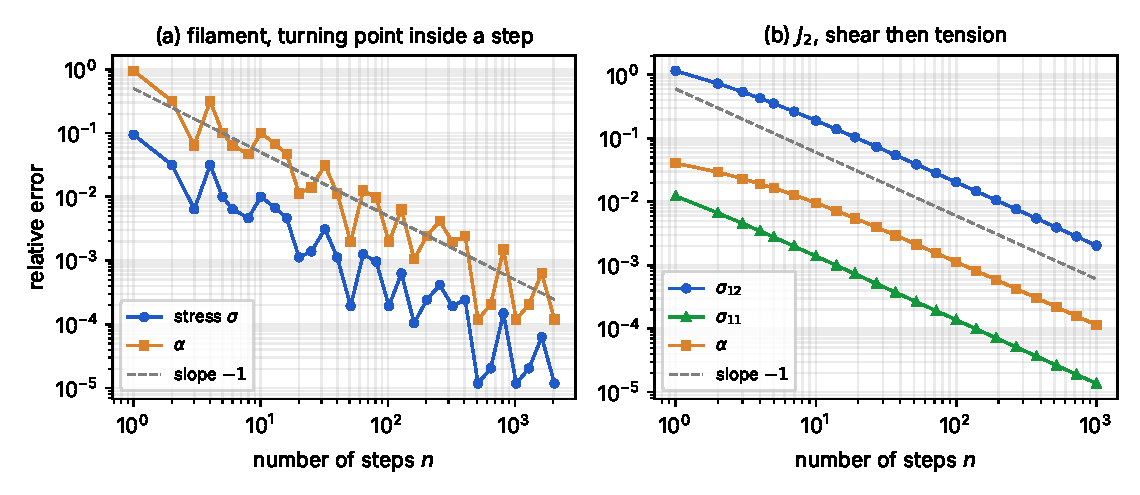
\includegraphics[width=\textwidth]{figures/ch5/errors.pdf}
\caption{Relative errors of the return map against the number of steps $n$.
(a) Filament of Exercise~\ref{exo:pn-nonmono}: the turning point of the
strain lies inside a step; the error decreases like $1/n$ on average, with
fluctuations due to the position of the turning point in its step.
(b) Shear then tension at fixed shear, Exercise~\ref{exo:pn-shear}: the
errors on $\sigma_{12}$, $\sigma_{11}$ and $\alpha$ are first order. The
dashed lines have the slope $-1$.}
\label{fig:pn-errors}
\end{figure}

\exercise{The plane-stress projected return}\label{exo:pn-ps}
\index{plane stress!exercise}%
(a) Show that $\mat{C}\mat{P}$ has the eigenvalues $E/(3(1-\nu))$, on
$(1,1,0)$, and $2\mu$, twice, and derive the decoupled update
\[
  \sigma_{11}+\sigma_{22}=\frac{(\sigma_{11}+\sigma_{22})^\trial}{1+\frac{E\dg}{3(1-\nu)}},\qquad
  (\sigma_{11}-\sigma_{22},\ \sigma_{12})=\frac{(\sigma_{11}-\sigma_{22},\ \sigma_{12})^\trial}{1+2\mu\dg},
\]
and the function $\varphi^2(\dg)$ of Box~5.5. (b) With $K=2$\,GPa, compute in
one step uniaxial tension to $\varepsilon_{11}=0.01$ and balanced biaxial
tension to $\varepsilon_{11}=\varepsilon_{22}=0.005$, and compare with the
closed forms. (c) Prescribe the in-plane strains: plane strain
($\varepsilon_{22}=0$) to $\varepsilon_{11}=0.01$. Is one step exact? The
script uses \texttt{plane\_stress\_return} (Box~5.5) of \texttt{ci\_core}.
\begin{solution}
(a) $\mat{C}$ and $\mat{P}$ commute and share the eigenvectors given in
Section~\ref{sec:pn-ps}; the products of their eigenvalues are
$\tfrac13E/(1-\nu)$, $2\mu$ and $2\mu$. In that basis
$(\mat{I}+\dg\mat{C}\mat{P})^{-1}$ is diagonal, which gives the update. Then
$\varphi^2=\vect{\sigma}\T\mat{P}\vect{\sigma}=\tfrac16(\sigma_{11}+\sigma_{22})^2+\tfrac12(\sigma_{11}-\sigma_{22})^2+2\sigma_{12}^2$.
(b) Uniaxial: $\alpha=\varepsilon^p_{11}$ and $\sigma=(\sY+K\varepsilon_{11})/(1+K/E)=267.326733$\,MPa;
biaxial: $\alpha=2\varepsilon^p_{11}$ and
$\sigma=(\sY+2K\varepsilon_{11})/(1+2K(1-\nu)/E)=266.272189$\,MPa. One step
gives both values to all digits: the stress direction is fixed by symmetry
($\sigma_{22}=0$, or $\sigma_{11}=\sigma_{22}$), and so is the normal.
(c) No. A proportional \emph{strain} path is not a proportional stress path:
the stress moves along the yield surface from the elastic ratio
$\sigma_{22}/\sigma_{11}=\nu$ towards the plane-strain value $\tfrac12$, as in
Exercise~\ref{exo:pl-sheet}. The one-step error is $6.9$\,MPa, and $0.22$,
$0.012$, $0.0010$\,MPa with 10, 100, 1000 steps. A code may reproduce the
tensile and bulge tests exactly at one step per increment and still need
small steps on a forming path.
\lstinputlisting[firstline=4]{python/examples/ch5/exo_plane_stress.py}
\end{solution}

\exercise{Hill anisotropy and the symmetry of the tangent}\label{exo:pn-hill}
\index{Hill criterion}\index{consistent tangent!symmetry}%
Hill's criterion~\cite{Hill1948} replaces the von Mises norm by
$\sigma_{eq}^2=\vect{\sigma}\cdot\mat{P}_H\vect{\sigma}$, with a symmetric positive
semi-definite matrix $\mat{P}_H$ that vanishes on hydrostatic stresses.
(a) Show that the backward Euler step with the associative flow
$\Delta\epsp=\dg\,\partial_{\sig}\sigma_{eq}$ is a closest-point projection, and
deduce that its consistent tangent is symmetric. (b) What happens if the flow
follows a different potential $g\ne\sigma_{eq}$ (for instance von Mises, while
the yield criterion is Hill's)? Check numerically by finite differences. The
script is self-contained: it does not use \texttt{ci\_core}, whose return maps
are written for von Mises and Tresca only.
\begin{solution}
(a) The projection property (Section~\ref{thm:pn-cpp}) holds for every convex $\Esig$: the elastic
domain of Hill's criterion is convex, and the step is the projection onto it.
By Section~\ref{thm:pn-W} the stress is the gradient of a convex potential
$W_n$, so its derivative is symmetric. In the linearization the rank-one term
is $(\bbC:\partial_{\sig}g)\otimes(\bbC:\partial_{\sig}f)/(\dots)$, symmetric
when $g=f$. (b) With $g\ne f$ the step is no longer a projection, there is no
potential, and the rank-one term is not symmetric. A general backward Euler
solver (Newton on $(\sig,\dg)$) and centred finite differences give, at a
generic strain, a relative asymmetry $\norm{\bbCalg-\bbCalg{}\T}/\norm{\bbCalg}$ of $10^{-9}$
(the finite-difference error) for von Mises and for associative Hill, and
$2.5\times10^{-2}$ for the non-associative model. The global stiffness is then
unsymmetric: a symmetric solver with the symmetrized tangent loses the
quadratic convergence, and the contractivity of
Section~\ref{thm:pn-contract} is lost.
\lstinputlisting[firstline=4]{python/examples/ch5/exo_hill.py}
\end{solution}

\framesub{Corners, stability and minimization}

\exercise{The Tresca corner}\label{exo:pn-tresca}
\index{Tresca criterion!corner (exercise)}%
In principal stresses take the two faces $f_a=\sigma_1-\sigma_3-\sY$ and
$f_b=\sigma_2-\sigma_3-\sY$, perfect plasticity, and Koiter's rule
$\Delta\epsp=\dg^a\tens N_a+\dg^b\tens N_b$. (a) Compute
$\tens N_i:\bbC:\tens N_j$ and the corner return. (b) Show that the corner is
the correct return if and only if $2f_b^\trial>f_a^\trial$, and interpret.
(c) With $\mu=76.92$\,GPa, sweep $f_b^\trial$ from $20$ to $5$\,MPa at
$f_a^\trial=20$\,MPa, with \texttt{tresca\_return} (Box~5.4) of
\texttt{ci\_core}.
\begin{solution}
(a) $\tens N_a=\ve_1\otimes\ve_1-\ve_3\otimes\ve_3$ and
$\tens N_b=\ve_2\otimes\ve_2-\ve_3\otimes\ve_3$ are deviatoric, so
$\bbC:\tens N_i=2\mu\tens N_i$, $\tens N_a:\bbC:\tens N_a=4\mu$ and
$\tens N_a:\bbC:\tens N_b=2\mu$. The two consistency conditions
$f_i^\trial-\sum_j\tens N_i:\bbC:\tens N_j\,\dg^j=0$ form a $2\times2$ system
of determinant $12\mu^2$, whose solution is in Box~5.4.
(b) The Kuhn--Tucker conditions require $\dg^b=(2f_b-f_a)/(6\mu)\ge0$ ($\dg^a\ge0$
holds since $f_a\ge f_b$). The trial state must lie in the cone of normals of
the vertex, where the closest point of $\Esig$ is the vertex itself. If
$\dg^b<0$, the face return applies, with $\dg^a=f_a/(4\mu)$.
(c) The corner is selected for $f_b=20$ ($\dg^a=\dg^b=4.33\times10^{-5}$) and $11$\,MPa
($\dg^b=4.3\times10^{-6}$); at $f_b=10$\,MPa, $\dg^b=0$, and below the face
return applies with $\dg^a=6.5\times10^{-5}$. The switch is continuous; the
tangent jumps. At the corner the plastic strain increment can be any positive
combination of $\tens N_a$ and $\tens N_b$ (Koiter's cone): the stress is
determined, the direction of flow depends on the trial state.
\lstinputlisting[firstline=4]{python/examples/ch5/exo_tresca.py}
\end{solution}

\exercise{Contractivity of the return map}\label{exo:pn-contract}
\index{B-stability!exercise}%
(a) Show that the return map never increases distances (Section~\ref{thm:pn-contract}) for perfect plasticity, where the
norm is $\norm{\sig}_E^2=\sig:\bbS:\sig$. (b) Show that forward Euler is not
contractive with the filament example of Section~\ref{sec:pn-stab}.
(c) Numerical test, perfect $J_2$ plasticity: state A is virgin; state B was
loaded plastically in tension ($\varepsilon_{11}=0.004$, lateral strains
$-0.002$) and brought back to zero strain. Both are then sheared to
$\gamma=0.03$ in $n$ steps. Follow the distance between the two stresses. The
script uses \texttt{radial\_return} of \texttt{ci\_core}, and a forward
Euler update written in the script.
\begin{solution}
(a) The trial stresses differ by $\sig_n-\sig'_n$, and the return map is the
projection onto $\Esig$ for $\scal{\cdot}{\cdot}_E$, which is non-expansive.
(b) With $\sigma=\sY$, $\sigma'=\sY-10$\,MPa and $\Delta\varepsilon=2.5\times10^{-4}$:
forward Euler gives $\sigma_\np=\sY$ and $\sigma'_\np=\sY+40$\,MPa, outside the
domain, and the distance grows from 10 to 40\,MPa; the return map gives
$\sigma_\np=\sigma'_\np=\sY$. (c) With backward Euler the distance decreases at
every step, for 4, 20 and 500 steps, from $0.52$ to $10^{-3}$, $7\times10^{-6}$
and $1.5\times10^{-7}$ (energy norm, $\sqrt{\mathrm{MPa}}$,
Figure~\ref{fig:pn-contract}): the two histories are forgotten, as plastic
flow forgets the initial state. Forward Euler leaves
the yield surface by up to $300\,\%$ with 4 steps and $2\,\%$ with 500 steps.
Contractivity is the discrete form of dissipation; a scheme without it can
create energy and is unstable in dynamics.
\lstinputlisting[firstline=4]{python/examples/ch5/exo_contract.py}
\end{solution}

\begin{figure}[h]
\centering
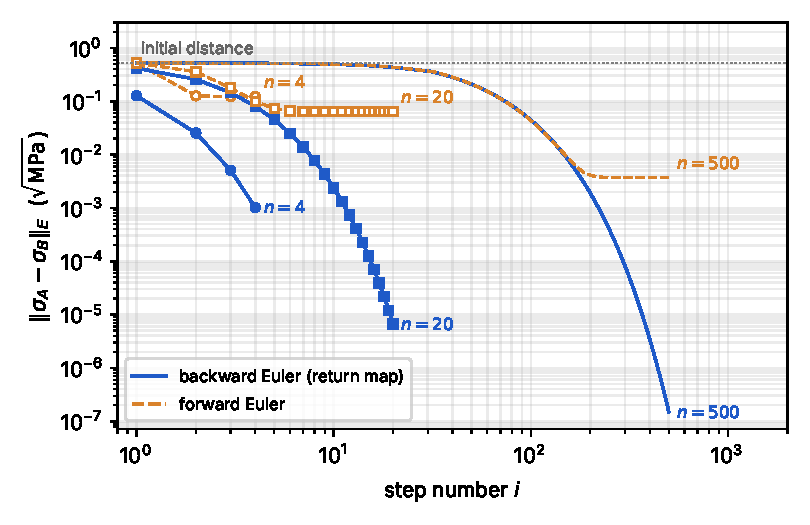
\includegraphics[width=0.66\textwidth]{figures/ch5/contract.pdf}
\caption{Exercise~\ref{exo:pn-contract}: energy distance between the stresses
of the virgin state A and of the pre-strained state B, both sheared to
$\gamma=0.03$ in $n=4$, $20$ and $500$ steps, against the step number (both
axes logarithmic). The return map (solid) decreases the distance at every
step, from $0.52\,\sqrt{\mathrm{MPa}}$ (dotted line) to zero. Forward Euler
(dashed) stalls at a distance that depends on the step size.}
\label{fig:pn-contract}
\end{figure}

\exercise{Viscoplastic updates as minimizations}\label{exo:pn-vp}
\index{viscoplasticity!exercise}%
(a) Show that the Perzyna step~\eqref{eq:pn-perzyna} is the minimizer of
$\displaystyle \tfrac12\norm{\vSig^\ast-\vSig^\trial}_E^2+\frac{\Delta t}{2\eta}\mac{f(\vSig^\ast)}^2$.
(b) For the filament without hardening, write the Perzyna and Duvaut--Lions
steps, and compare them with the exact relaxation~\eqref{eq:pl-relax} for a
strain held fixed after a jump.
\begin{solution}
(a) The function is strictly convex ($\mac{f}^2$ is convex for convex $f$).
Its stationarity condition is
$\tensf{G}^{-1}(\vSig-\vSig^\trial)+\frac{\Delta t}{\eta}\mac{f(\vSig)}\partial f(\vSig)=\vzero$,
i.e.\ $\vSig=\vSig^\trial-\tensf{G}\Delta\vz$ with
$\Delta\vz=\frac{\Delta t}{\eta}\mac{f}\partial f$: the backward Euler step. As
$\eta\to0$ the penalty forces $f\le0$ and the projection is recovered.
(b) Without hardening the two models coincide in one dimension ($\tau=\eta/E$).
For $\sigma^\trial>\sY$ both give
$\sigma_\np-\sY=(\sigma^\trial-\sY)/(1+\Delta t/\tau)$, while the exact
solution is $(\sigma^\trial_\np-\sY)e^{-\Delta t/\tau}$ after the jump. The ratio
$1/(1+r)$ approximates $e^{-r}$ to first order, and both tend to zero as
$r\to\infty$: the scheme is stable for every step and relaxes to the yield
surface.
\end{solution}

\exercise{Incremental potential of \texorpdfstring{$J_2$}{J2} plasticity}\label{exo:pn-W}
\index{incremental potential!exercise}%
(a) Derive~\eqref{eq:pn-WJ2} for combined linear hardening. (b) Show that its
gradient is $\sig_\np$ and its Hessian $\bbCalg$, and find the eigenvalues of
$\bbCalg$. (c) Deduce that $W_n$ is strongly convex if $K+H>0$.
\begin{solution}
(a) $\Delta\vz=\dg\,(\tn,\sqrt{2/3},\tn)$ for $(\epsp,\alpha,\valpha_{\mathrm{kin}})$,
$\tensf{G}=\diag(\bbC,K,\tfrac23H\bbI)$, so that
$\Delta\vz\cdot\tensf{G}\Delta\vz=\dg^2(2\mu+\tfrac23K+\tfrac23H)=h\dg^2=\mac{f^\trial}^2/h$;
insert in item (b) of Section~\ref{thm:pn-W}. (b) In the plastic region,
$\partial f^\trial/\partial\eps=2\mu\tn$ and
$\partial\tn/\partial\eps=\frac{2\mu}{\norm{\teta^\trial}}(\bbIdev-\tn\otimes\tn)$.
The gradient is $\sig^\trial-2\mu\frac{f^\trial}{h}\tn=\sig_\np$; differentiating
again gives~\eqref{eq:pn-calg}. The eigenvalues are $3\kappa$,
$2\mu(K+H)/(3\mu+K+H)$ and $2\mu\theta$ (multiplicity four).
(c) Since $f^\trial\le\norm{\teta^\trial}$, $\theta\ge1-2\mu/h=(K+H)/(3\mu+K+H)$:
all eigenvalues are bounded below by
$m=\min\{3\kappa,\,2\mu(K+H)/(3\mu+K+H)\}>0$, in the elastic region too.
The elastic region of $\eps$-space is convex, so a segment crosses its
boundary at most twice, and the gradient is strongly monotone along every
segment. Without hardening $m=0$ and the potential grows linearly.
\end{solution}

\framesub{A finite element code}

\exercise{The thick-walled cylinder by finite elements}\label{exo:pn-fem}
\index{thick-walled cylinder!finite elements}%
Write an axisymmetric plane-strain finite element code for the cylinder of
Exercise~\ref{exo:pl-cyl} (linear elements, unknown $u(r)$, strains
$(\dd u/\dd r,\ u/r,\ 0)$), with the radial return of Box~5.2 and the global
Newton method of Box~5.3 (Algorithm~\ref{alg:pn-fem}). For perfect plasticity,
$\sY=250$\,MPa, $b=2a$, apply $p=0.8\,p_L$ and $0.95\,p_L$ with
$\displaystyle p_L=\frac{2\sY}{\sqrt3}\ln\frac ba$, and compare the radius of the plastic
zone with the Tresca-type solution of Exercise~\ref{exo:pl-cyl}. The module
\texttt{ci\_fem} (page~\pageref{sec:pn-aux}) is such a code, built on
\texttt{radial\_return} of \texttt{ci\_core}; the test program below calls its
functions \texttt{solve} and \texttt{p\_of\_c}.
\begin{algorithm}[H]
\caption{Incremental Newton solver (Box~5.3)}\label{alg:pn-fem}
\begin{algorithmic}[1]
\Require mesh, material, load steps $p_1<\dots<p_N$, tolerance $\epsilon$
\Ensure nodal displacements $\mat{u}_n$, internal variables $\vz_n$ at the Gauss points
\State $\mat{u}\gets\mat{0}$;\ \ $\vz_0\gets\vzero$ at every Gauss point
\For{$n=0,\dots,N-1$}
  \Repeat
    \State $\mat{F}^{\mathrm{int}}\gets\mat{0}$;\ \ $\mat{K}\gets\mat{0}$
    \For{each element $e$ and Gauss point $g$}
      \State $(\sig,\vz^{\ast}_g,\bbCalg)\gets\textsc{RadialReturn}(\mat{B}_g\mat{u},\ \vz_{n,g})$ \Comment{from $\vz_n$}
      \State $\mat{F}^{\mathrm{int}}\mathrel{+}=w_g\mat{B}_g\T\sig$;\ \ $\mat{K}\mathrel{+}=w_g\mat{B}_g\T\mat{C}^{\mathrm{alg}}\mat{B}_g$
    \EndFor
    \State $\mat{R}\gets\mat{F}^{\mathrm{ext}}(p_\np)-\mat{F}^{\mathrm{int}}$
    \If{$\norm{\mat{R}}>\epsilon\norm{\mat{F}^{\mathrm{ext}}}$} \ $\mat{u}\gets\mat{u}+\mat{K}^{-1}\mat{R}$ \EndIf
  \Until{$\norm{\mat{R}}\le\epsilon\norm{\mat{F}^{\mathrm{ext}}}$}
  \State $\vz_{\np,g}\gets\vz^{\ast}_g$ at every Gauss point \Comment{accept the step}
\EndFor
\end{algorithmic}
\end{algorithm}
\begin{solution}
With 200 elements and 20 steps, $p_L=200.09$\,MPa. At $0.8\,p_L$ the plastic
zone reaches $c=131.0$\,mm against $130.8$\,mm, and at $0.95\,p_L$ $c=165.5$
against $164.0$\,mm. The small difference is not a discretization error: the
closed form assumes $\sigma_\theta-\sigma_r=2\sY/\sqrt3$, which is exact for
von Mises only when $\sigma_z$ is the mean of $\sigma_r$ and $\sigma_\theta$,
i.e.\ for incompressible plastic flow; in the elastic--plastic regime the
elastic compressibility makes $\sigma_z$ differ slightly. Near $p_L$ the bore
displacement grows quickly and Newton needs more iterations; at $p_L$ the
tangent stiffness becomes singular. The weight of a Gauss point is
$w_g=r_g\,L_e$ (the factor $2\pi$ cancels). Over the whole range from the
first yield, at $p=0.541\,p_L$, to $0.98\,p_L$, the computed radius follows
the closed form (Figure~\ref{fig:pn-cylzone}); the gap stays below $0.7$\,mm
up to $0.9\,p_L$ and grows to $2.6$\,mm at $0.98\,p_L$. Near $p_L$ the curve
$c(p)$ is steep, and a small difference in pressure, due to the
approximation on $\sigma_z$ discussed above, becomes a large difference in
radius.
Compare with similar computations performed in standard finite element codes,
for example Cast3M or FEniCS.
\lstinputlisting[firstline=90]{python/examples/ch5/ci_fem.py}
\end{solution}

\begin{figure}[h]
\centering
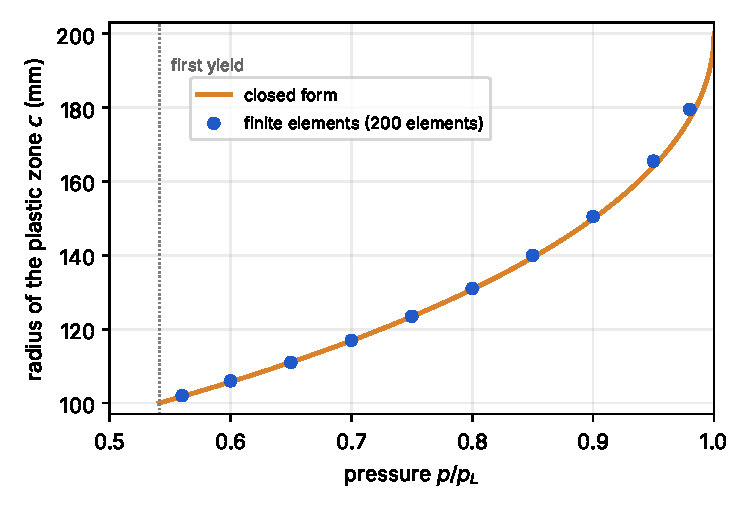
\includegraphics[width=0.6\textwidth]{figures/ch5/cylinder_zone.pdf}
\caption{Exercise~\ref{exo:pn-fem}: radius $c$ of the plastic zone of the
thick-walled cylinder ($b=2a=200$\,mm, perfect $J_2$ plasticity) against the
pressure. Finite elements (200 elements, 20 load steps per computation)
against the closed form
$p=k\ln(c/a)+\tfrac k2\bigl(1-c^2/b^2\bigr)$, $k=2\sY/\sqrt3$. The plastic
zone appears at $p=0.541\,p_L$ and reaches the outer radius at $p_L$.}
\label{fig:pn-cylzone}
\end{figure}

%======================================================================
\begin{chapterbib}{99}
\bibitem{BauschkeCombettes2017} H.~H.~Bauschke, P.~L.~Combettes, \emph{Convex Analysis and Monotone Operator Theory in Hilbert Spaces}, 2nd ed., Springer, 2017.
\bibitem{deSouzaNeto2008} E.~A.~de Souza Neto, D.~Peri\'c, D.~R.~J.~Owen, \emph{Computational Methods for Plasticity: Theory and Applications}, Wiley, 2008.
\bibitem{Hill1948} R.~Hill, A theory of the yielding and plastic flow of anisotropic metals, \emph{Proc. R. Soc. Lond. A} 193 (1948) 281--297.
\bibitem{KondoMaitournam2023b} D.~Kondo, H.~Maitournam, Thermodynamics of irreversible processes: formulation of constitutive models, Chapter~2 in J.~Besson et al., \emph{MEALOR II: Damage Mechanics and Local Approach to Fracture}, 2023, 5--38, doi:10.5281/zenodo.10125170.
\bibitem{KriegKey1976} R.~D.~Krieg, S.~W.~Key, Implementation of a time independent plasticity theory into structural computer programs, in J.~A.~Stricklin, K.~J.~Saczalski (eds.), \emph{Constitutive Equations in Viscoplasticity: Computational and Engineering Aspects}, AMD-20, ASME, 1976, 125--137.
\bibitem{KriegKrieg1977} R.~D.~Krieg, D.~B.~Krieg, Accuracies of numerical solution methods for the elastic--perfectly plastic model, \emph{J. Pressure Vessel Technol.} 99 (1977) 510--515.
\bibitem{Maitournam2012b} H.~Maitournam, \emph{Mat\'eriaux et structures an\'elastiques}, Presses de l'\'Ecole polytechnique, 2012.
\bibitem{Miehe2002} C.~Miehe, Strain-driven homogenization of inelastic microstructures and composites based on an incremental variational formulation, \emph{Int. J. Numer. Meth. Engng} 55 (2002) 1285--1322.
\bibitem{Moreau1965} J.-J.~Moreau, Proximit\'e et dualit\'e dans un espace hilbertien, \emph{Bull. Soc. Math. France} 93 (1965) 273--299.
\bibitem{OrtizPopov1985} M.~Ortiz, E.~P.~Popov, Accuracy and stability of integration algorithms for elastoplastic constitutive relations, \emph{Int. J. Numer. Meth. Engng} 21 (1985) 1561--1576.
\bibitem{OrtizSimo1986} M.~Ortiz, J.~C.~Simo, An analysis of a new class of integration algorithms for elastoplastic constitutive relations, \emph{Int. J. Numer. Meth. Engng} 23 (1986) 353--366.
\bibitem{OrtizStainier1999} M.~Ortiz, L.~Stainier, The variational formulation of viscoplastic constitutive updates, \emph{Comput. Methods Appl. Mech. Engrg.} 171 (1999) 419--444.
\bibitem{SimoGovindjee1991} J.~C.~Simo, S.~Govindjee, Non-linear B-stability and symmetry preserving return mapping algorithms for plasticity and viscoplasticity, \emph{Int. J. Numer. Meth. Engng} 31 (1991) 151--176.
\bibitem{SimoHughesCI} J.~C.~Simo, T.~J.~R.~Hughes, \emph{Computational Inelasticity}, Springer, 1998.
\bibitem{SimoKennedyGovindjee1988} J.~C.~Simo, J.~G.~Kennedy, S.~Govindjee, Non-smooth multisurface plasticity and viscoplasticity. Loading/unloading conditions and numerical algorithms, \emph{Int. J. Numer. Meth. Engng} 26 (1988) 2161--2185.
\bibitem{SimoTaylor1985} J.~C.~Simo, R.~L.~Taylor, Consistent tangent operators for rate-independent elastoplasticity, \emph{Comput. Methods Appl. Mech. Engrg.} 48 (1985) 101--118.
\bibitem{SimoTaylor1986} J.~C.~Simo, R.~L.~Taylor, A return mapping algorithm for plane stress elastoplasticity, \emph{Int. J. Numer. Meth. Engng} 22 (1986) 649--670.
\bibitem{Wilkins1964} M.~L.~Wilkins, Calculation of elastic-plastic flow, in B.~Alder, S.~Fernbach, M.~Rotenberg (eds.), \emph{Methods in Computational Physics}, Vol.~3, Academic Press, 1964, 211--263.
\end{chapterbib}
